\chapter{User Documentation}
\label{ch:user}

This chapter provides comprehensive documentation for users of the Solar Energy Monitoring and Control System. The documentation is organized to help different user types quickly find the information they need.

\section{System Overview}
\label{sec:system-overview}

\subsection{What is the Solar Energy Monitoring and Control System?}
\label{subsec:system-description}

The Solar Energy Monitoring and Control System is a web-based platform that enables real-time monitoring and management of solar installations using Pay-As-You-Go (PAYG) financing models. Key capabilities include: real-time energy production and consumption tracking with automated summaries, flexible installment payment management with multiple frequency options, tamper detection and security monitoring, remote service control for payment compliance, role-based user access (Admin/Customer), and comprehensive analytics dashboards.

\subsection{Who Should Use This Documentation}
\label{subsec:target-audience}

\textbf{Primary Users:} System Administrators (platform configuration, user management) and Solar Installation Customers (energy monitoring, payment management).

\textbf{Prerequisites:} Administrators need web application management skills; Customers need basic computer literacy and email access.

\subsection{System Components}
\label{subsec:system-components}

The system consists of four main components: (1) \textbf{Backend API} -- Spring Boot application providing REST APIs, WebSocket endpoints for real-time updates, business logic, and authentication; (2) \textbf{Frontend Web Application} -- Next.js-based responsive interface with separate dashboards for administrators and customers; (3) \textbf{PostgreSQL Database} -- Stores user data, energy readings, payments, tamper events, and operational logs; (4) \textbf{IoT Device/Simulator} -- Python-based component representing Raspberry Pi devices installed at solar sites to collect and transmit energy data and tamper alerts (simulator provided for testing without physical hardware). The system implements role-based access control with two roles (Table~\ref{tab:role-privileges}).

\begin{table}[h]
    \centering
    \caption{Access privileges by user role}
    \label{tab:role-privileges}
    \begin{tabular}{|l|c|c|}
        \hline
        \textbf{Feature} & \textbf{Admin} & \textbf{Customer} \\
        \hline
        User Management & Full & Self Only \\
        Energy Monitoring & Full & Own Only \\
        Payment Processing & Full & Own Only \\
        Security Alerts & Full & Limited \\
        System Configuration & Full & No \\
        Reports & Full & Limited \\
        \hline
    \end{tabular}
\end{table}

\section{Quick Start Guide}
\label{sec:quick-start}

\subsection{System Requirements}
\label{subsec:system-requirements}

\subsubsection{For End Users (Customers)}
\label{subsubsec:end-user-requirements}

Requirements: Modern computer/tablet/smartphone, stable internet (1+ Mbps), active email account. Supported browsers: Chrome 88+, Firefox 85+, Edge 88+, Safari 14+. JavaScript and cookies must be enabled. Minimum resolution: 1280$\times$768.

\subsubsection{For System Administrators}
\label{subsubsec:admin-requirements}

Since the system runs in Docker containers, administrators only need Docker Desktop (or Docker Engine with Docker Compose) installed on their host system. Recommended hardware: at least 8GB RAM and sufficient disk space for container images and database storage. All other dependencies (Java, PostgreSQL, etc.) are bundled within the containers.

\subsection{Account Access}
\label{subsec:account-access}

\subsubsection{Getting Your Account}
\label{subsubsec:getting-account}

\textbf{For Customers:} Your solar installation provider (administrator) will create your account and you will receive an email with an activation link. Click the link, then set your password following the requirements: minimum 8 characters including at least one uppercase letter, one lowercase letter, one number, and one special character.

\textbf{For Administrators:} The administrator account is automatically created during system deployment using credentials configured in the environment file. On first login, you must change this default password to a secure one.

\subsubsection{Logging In}
\label{subsubsec:logging-in}

Navigate to system URL, enter email and password, click "Sign In". Figure~\ref{fig:login} shows the login interface.

\begin{figure}[htbp]
    \centering
    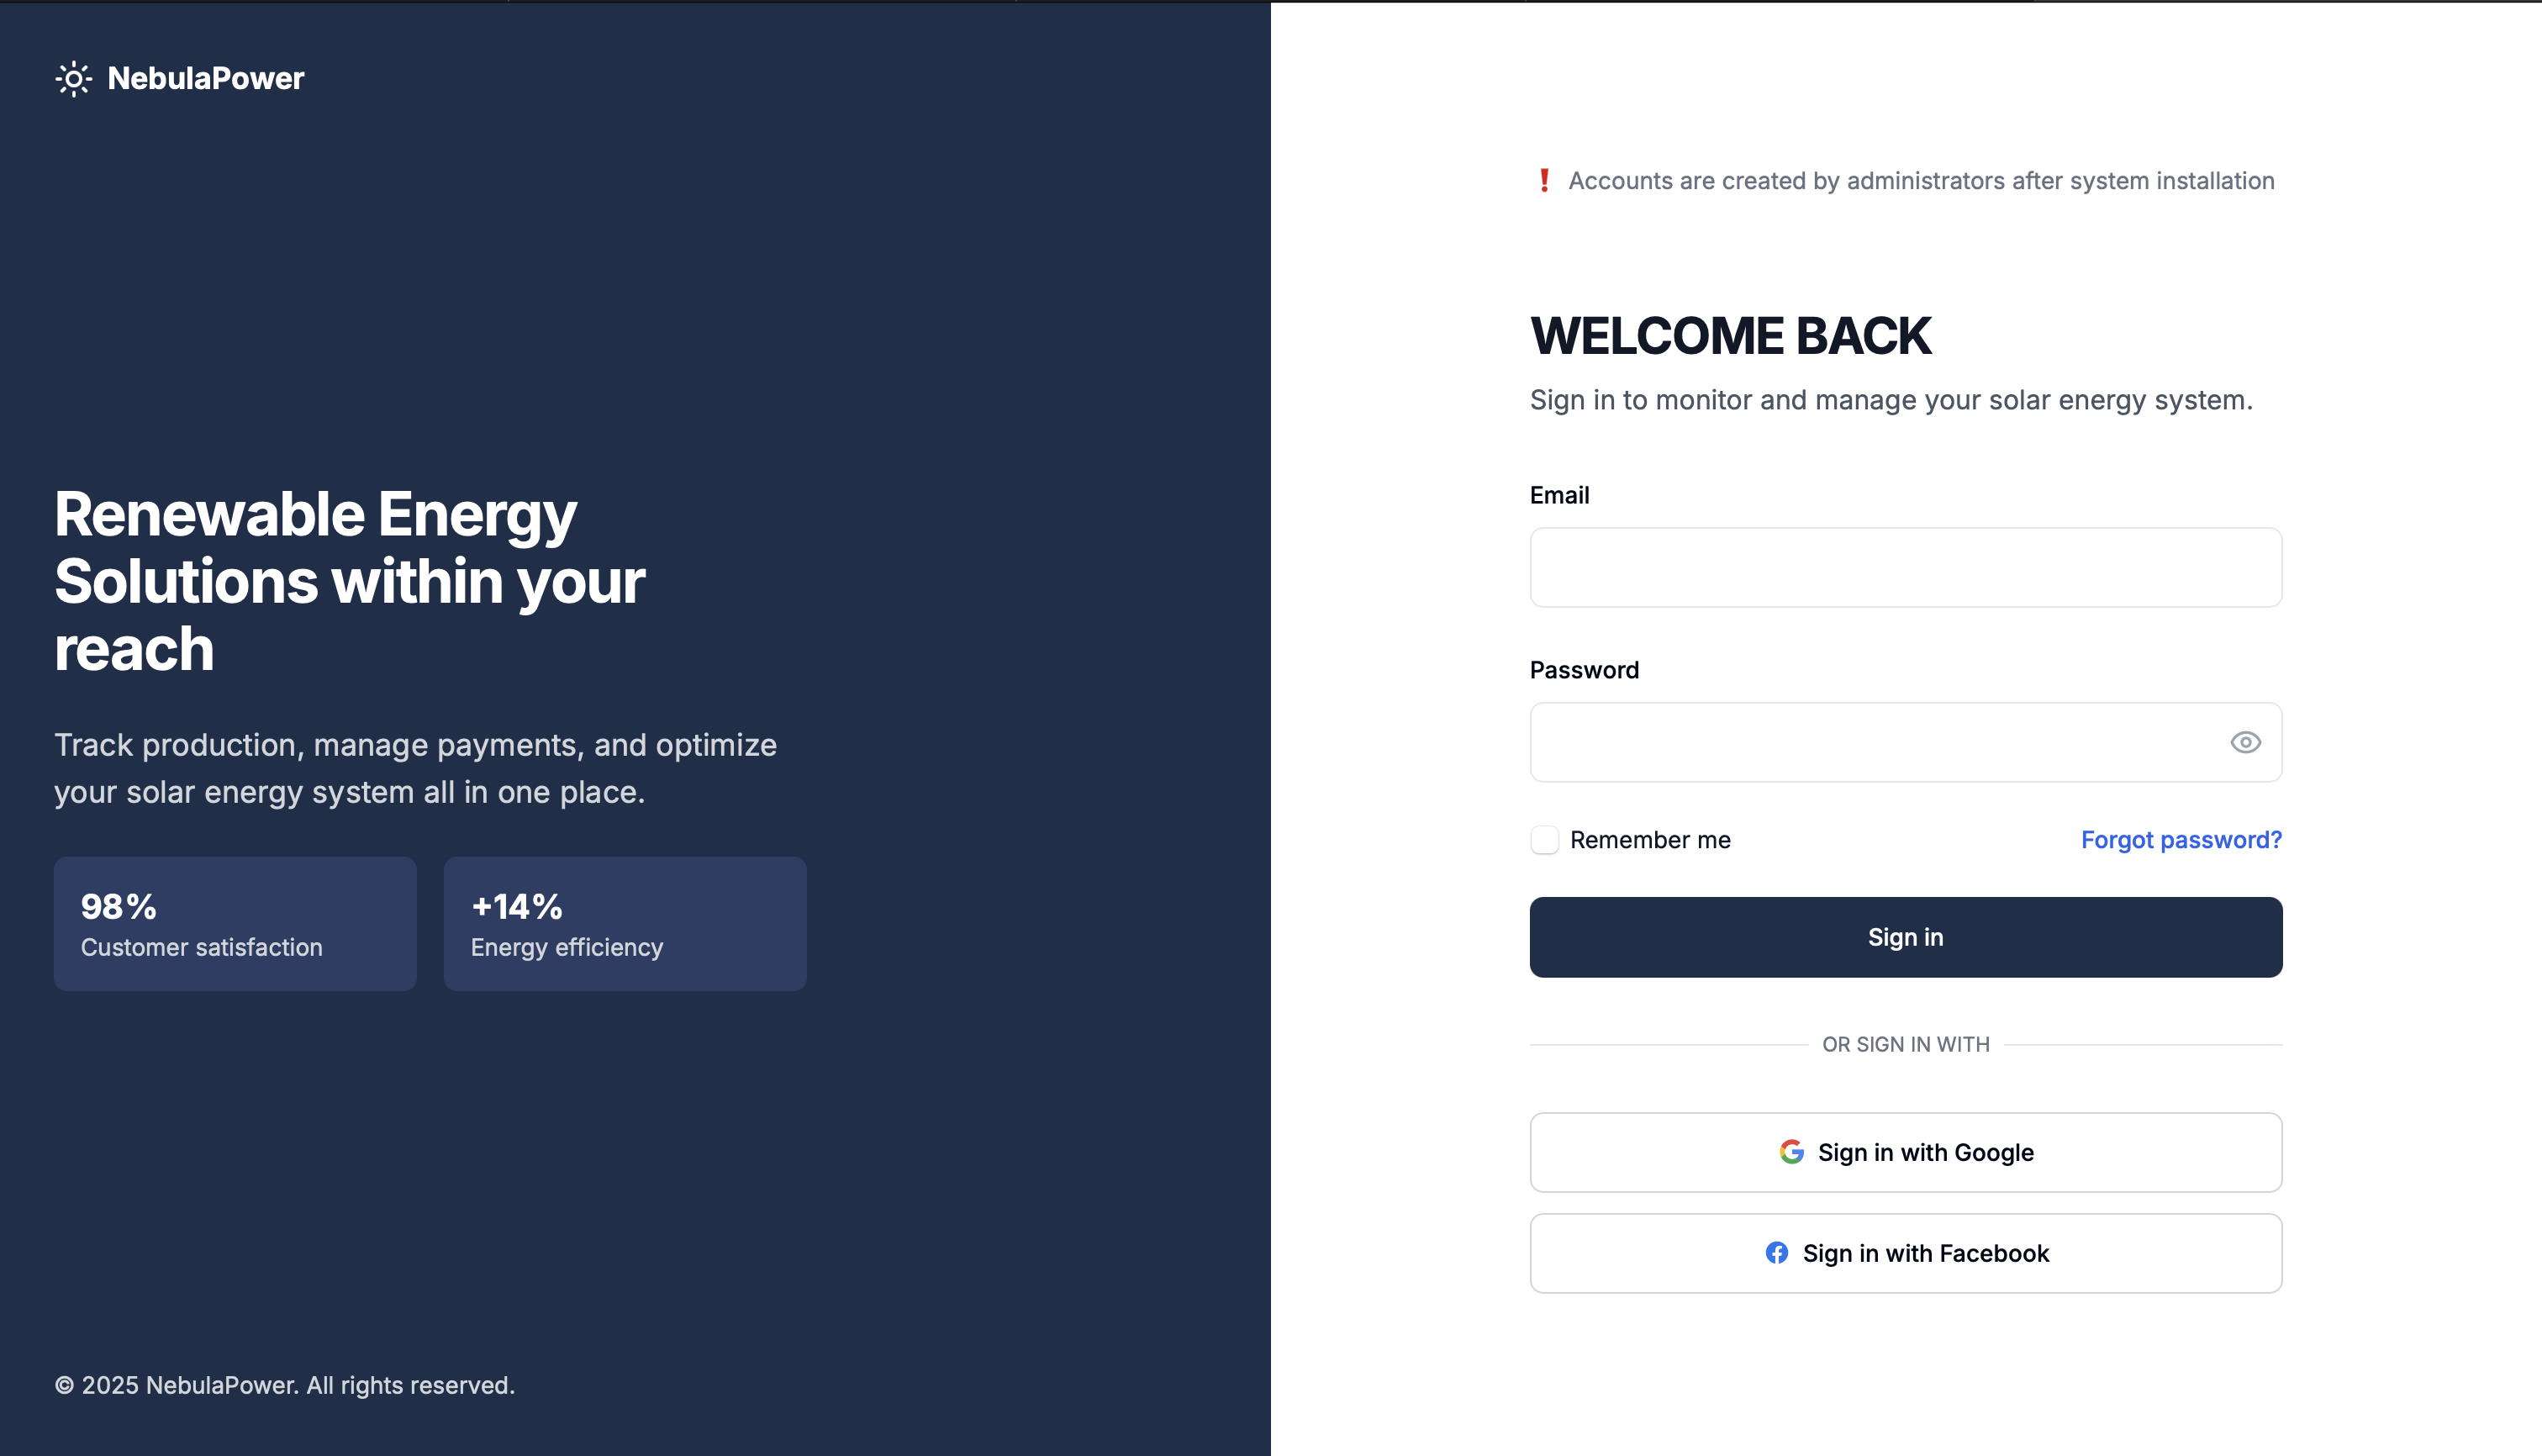
\includegraphics[width=0.9\textwidth]{images_2/login_pg.png}
    \caption{User login interface}
    \label{fig:login}
\end{figure}

\subsubsection{Password Management}
\label{subsubsec:password-management}

\textbf{Note}: Email functionality is simulated for demonstration only.

\textbf{Reset:} Click "Forgot Password," enter email, follow reset link. \textbf{Change:} Profile Settings $\rightarrow$ enter current and new passwords $\rightarrow$ save.

\section{User Interface Guide}
\label{sec:ui-guide}

\subsection{Technical Requirements}

The web interface works with modern browsers including Chrome, Firefox, Edge, Safari, and Opera. You need JavaScript and cookies enabled, and a screen resolution of at least 1280$\times$768 pixels. A stable internet connection is required for accessing the system and receiving real-time updates.

\section{Installation and Setup Guide}
\label{sec:installation-setup}

\subsection{Prerequisites}
\label{subsec:prerequisites}

Before installing, ensure you have Docker Desktop (version 4.0 or newer) or Docker Engine (version 20.10 or newer) with Docker Compose (version 2.0 or newer) installed on your system. Your computer should have at least 4GB of RAM available, though 8GB is recommended for better performance.

\subsection{Quick Docker Installation}
\label{subsec:docker-installation}

\textbf{1) Clone and prepare environment}

Open a terminal or command-line interface and navigate to the folder where you want to install the system, then run:

\begin{verbatim}
git clone https://github.com/2001J/nebular-power.git
cd nebular-power
cp .env.template .env     # create .env (copied from .env.template)
\end{verbatim}

Open the \texttt{.env} file and set your administrator credentials (\texttt{ADMIN\_EMAIL}, \texttt{ADMIN\_PASSWORD}) and a secure random string for \texttt{JWT\_SECRET}. The database settings have sensible defaults that you can change if needed.

\textbf{2) Start services}
\begin{verbatim}
docker compose up -d
\end{verbatim}

This command starts three containers running the database, backend API, and frontend application. Wait a minute or two for the database to initialize.

\textbf{3) Access the application}
\begin{itemize}
    \item Web Interface: \url{http://localhost:3000}
    \item API Documentation: \url{http://localhost:8080/swagger-ui.html}
\end{itemize}

Log in using the administrator credentials you configured. You should change the password on first login for security.

\subsection{Configuration}
\label{subsec:system-configuration}

All system settings are managed through the \texttt{.env} file (copied from \texttt{.env.template}). The most important settings include your administrator account details for initial access, authentication secrets for security, database connection settings (with defaults provided), email server configuration for notifications (optional for local testing), and the system profile which determines whether to use the development or production database.

For production deployment, use strong passwords and secrets, and configure a real email service for sending notifications.

\subsection{Device Simulation}
\label{subsec:device-simulation}

To simulate IoT devices sending energy data and tamper alerts, you need to set up the Python simulator. This can run on the same machine as your Docker containers (using \texttt{localhost:8080} as the backend URL) or on a separate device like a Raspberry Pi (using the IP address of the machine running the backend).

\textbf{Setup steps:}

Navigate to the simulation folder and create a virtual environment:
\begin{verbatim}
cd pi_simulation
python3 -m venv venv
source venv/bin/activate      # On Windows: venv\Scripts\activate
\end{verbatim}

Install dependencies:
\begin{verbatim}
pip3 install -r requirements.txt
\end{verbatim}

Edit \texttt{config.json} to set the backend URL:
\begin{itemize}
    \item For same machine: \texttt{http://localhost:8080}
    \item For Raspberry Pi or separate device: \texttt{http://[BACKEND\_IP]:8080} (replace \texttt{[BACKEND\_IP]} with the actual IP address)
\end{itemize}

Run the simulator:
\begin{verbatim}
python3 main.py
\end{verbatim}

\subsection{Verification and Management}
\label{subsec:verification}

After installation, verify everything is running by checking container status with \texttt{docker compose ps}. You can view logs using \texttt{docker compose logs -f backend} to monitor the application. Open the web interface and sign in with your administrator credentials to confirm successful deployment.

If you encounter port conflicts, adjust the \texttt{POSTGRES\_HOST\_PORT} setting in your \texttt{.env} file. If the database takes time to initialize, wait 2--3 minutes and check the database logs with \texttt{docker compose logs postgres}. For authentication issues, verify that your database credentials in \texttt{.env} match correctly.

To manage the system, use \texttt{docker compose up -d} to start services, \texttt{docker compose down} to stop everything, \texttt{docker compose restart backend} to restart a specific service, and \texttt{docker compose logs -f backend} to monitor logs in real-time.

\subsection{Account Setup and Access}
\label{subsec:account-setup}

Administrators can create customer accounts through the Customer Management interface. New customers receive an activation email and set their own password following security requirements (minimum 8 characters with uppercase, lowercase, numbers, and special characters). See Figure~\ref{fig:customer-onboarding}.

\begin{figure}[htbp]
    \centering
    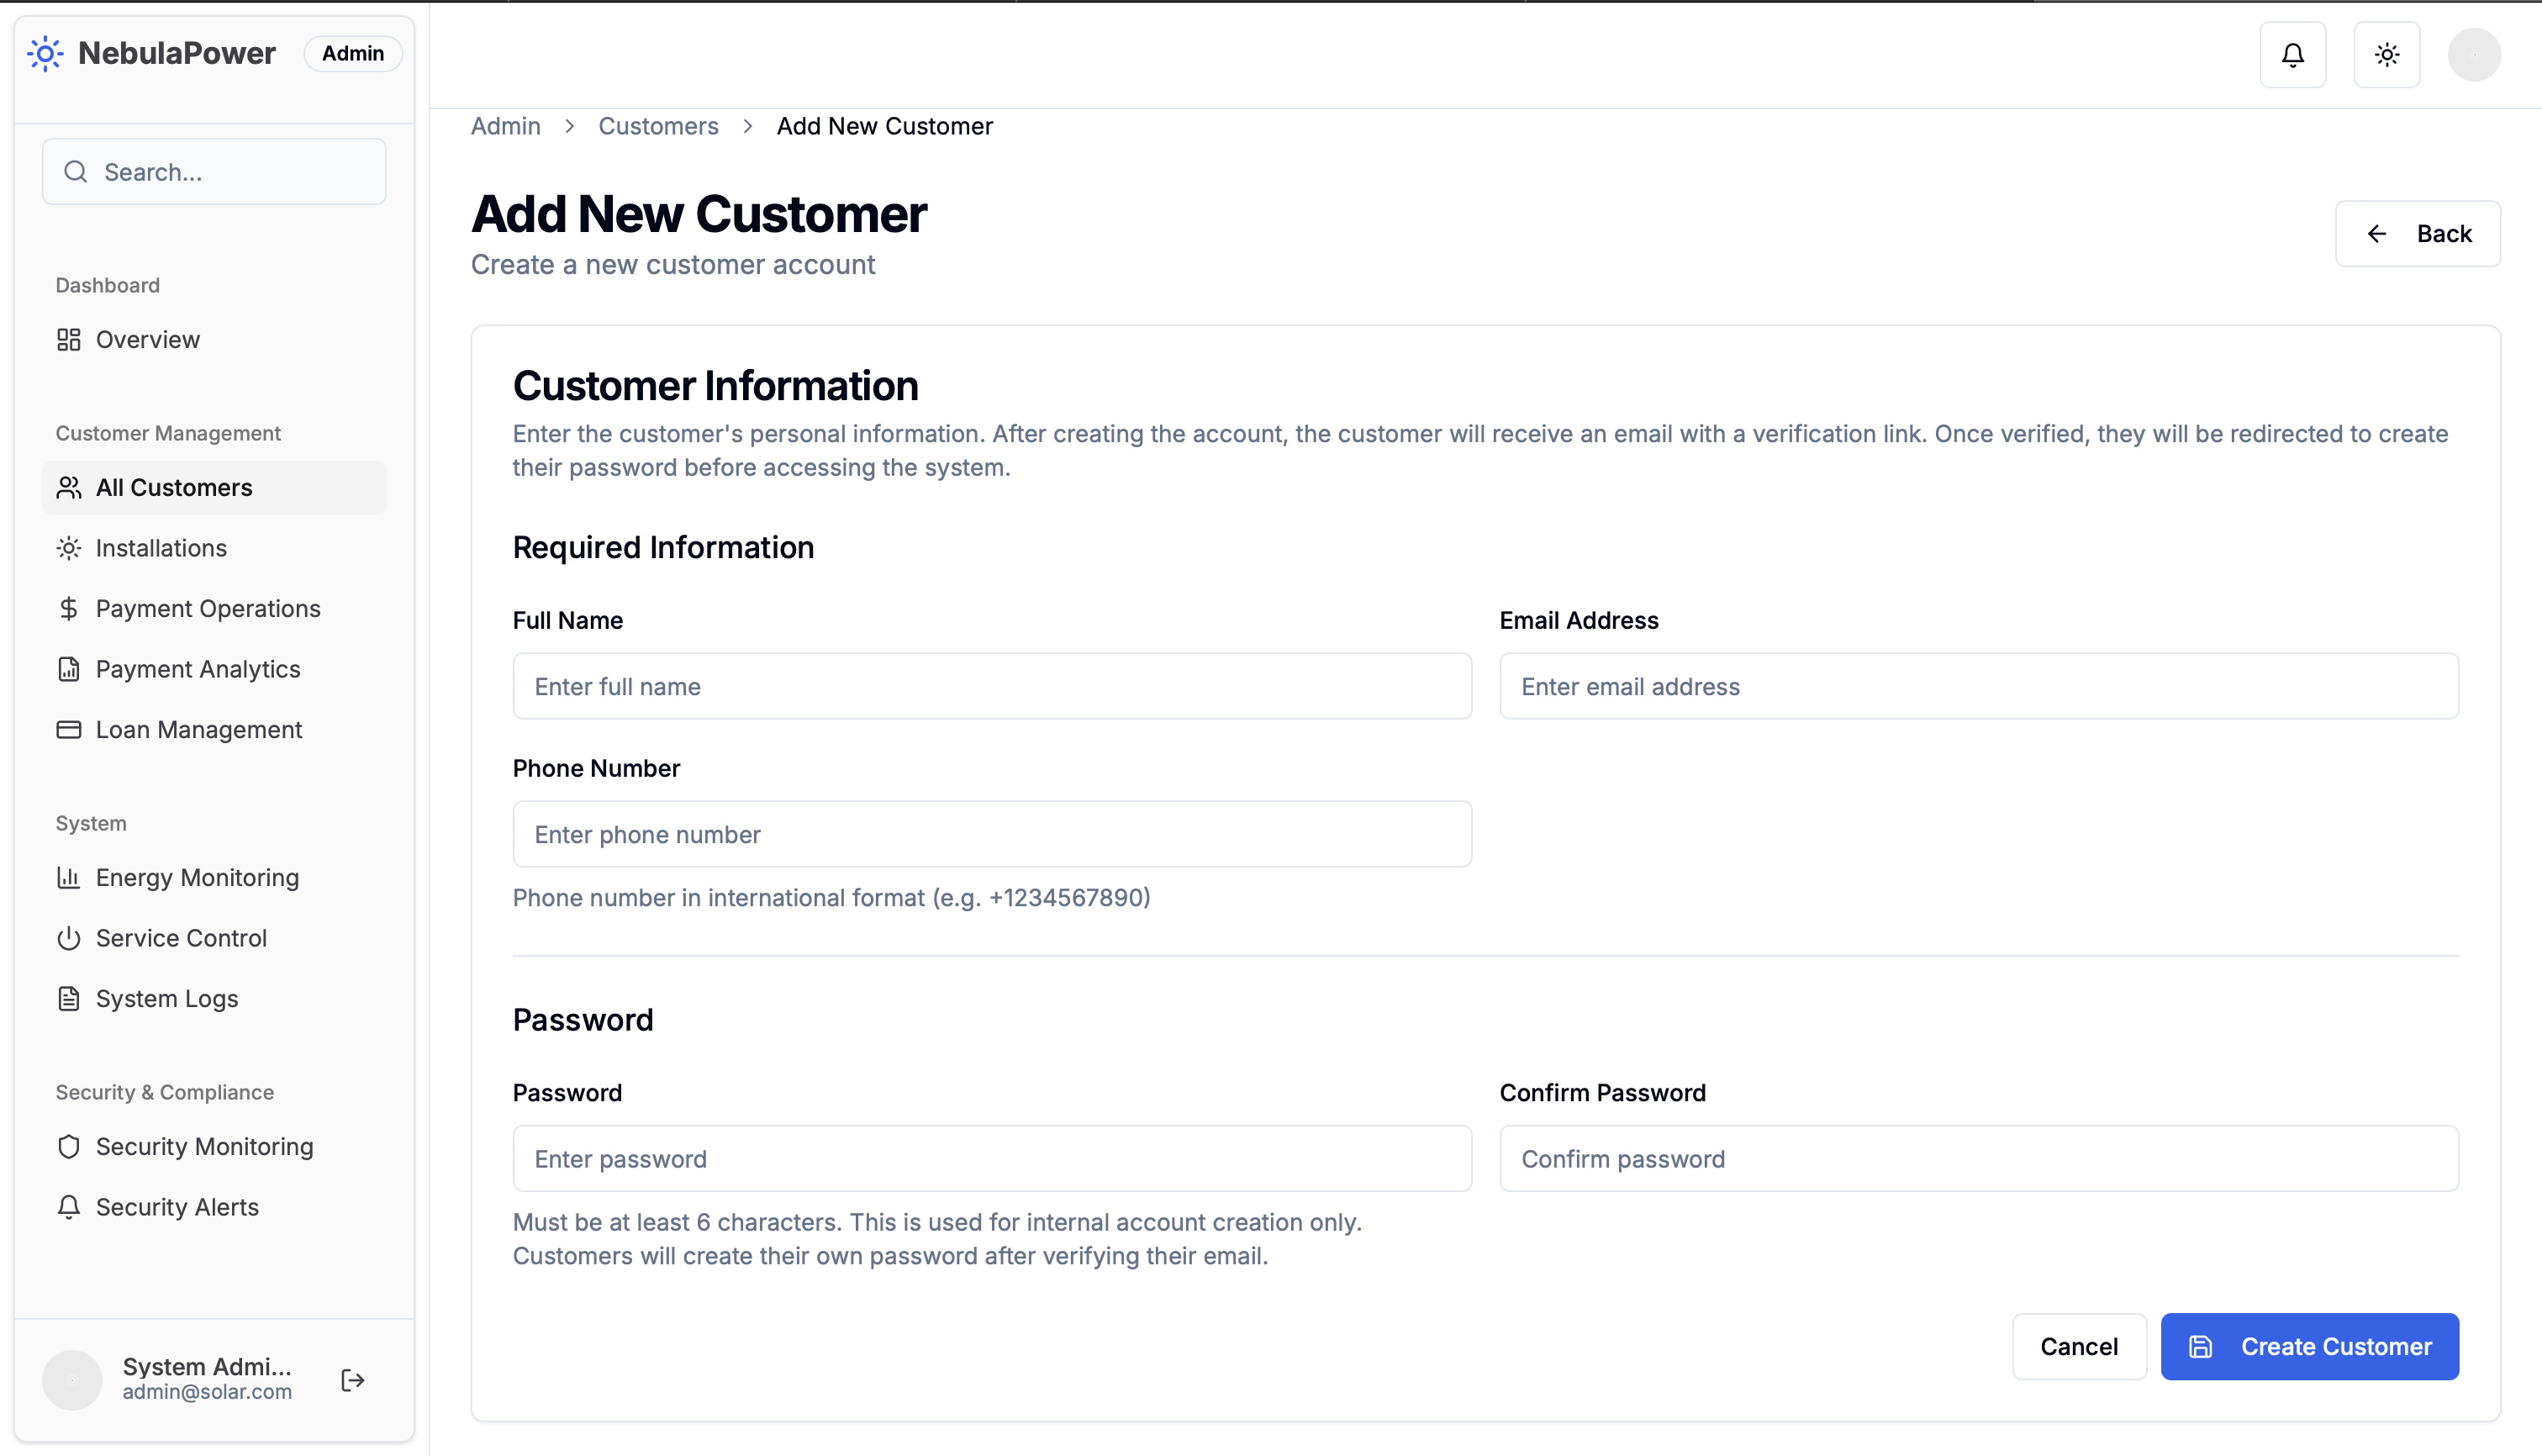
\includegraphics[width=0.9\textwidth]{images_2/customer_onboard.png}
    \caption{Customer onboarding interface (admin view)}
    \label{fig:customer-onboarding}
\end{figure}

\textbf{Login:} Navigate to login page, enter email/password, click "Sign In."

\textbf{Password Management:} Reset via "Forgot Password" link; change in profile settings.

\section{Dashboard Interface Guide}
\label{sec:dashboard-guide}

This section provides a detailed overview of the Solar Energy Monitoring and Control System's user interface, highlighting key screens and navigation patterns.

\subsection{Dashboard Overview}
\label{subsec:dashboard-overview}

The dashboard is your main workspace after logging in. The interface you see depends on your user role.

\subsubsection{Administrator Dashboard}
\label{subsubsec:admin-dashboard}

Navigation: Dashboard (system overview), Customer Management, Payment Operations, System (energy, logs), Security \& Compliance. See Figure~\ref{fig:admin-dashboard}.

\begin{figure}[h]
    \centering
    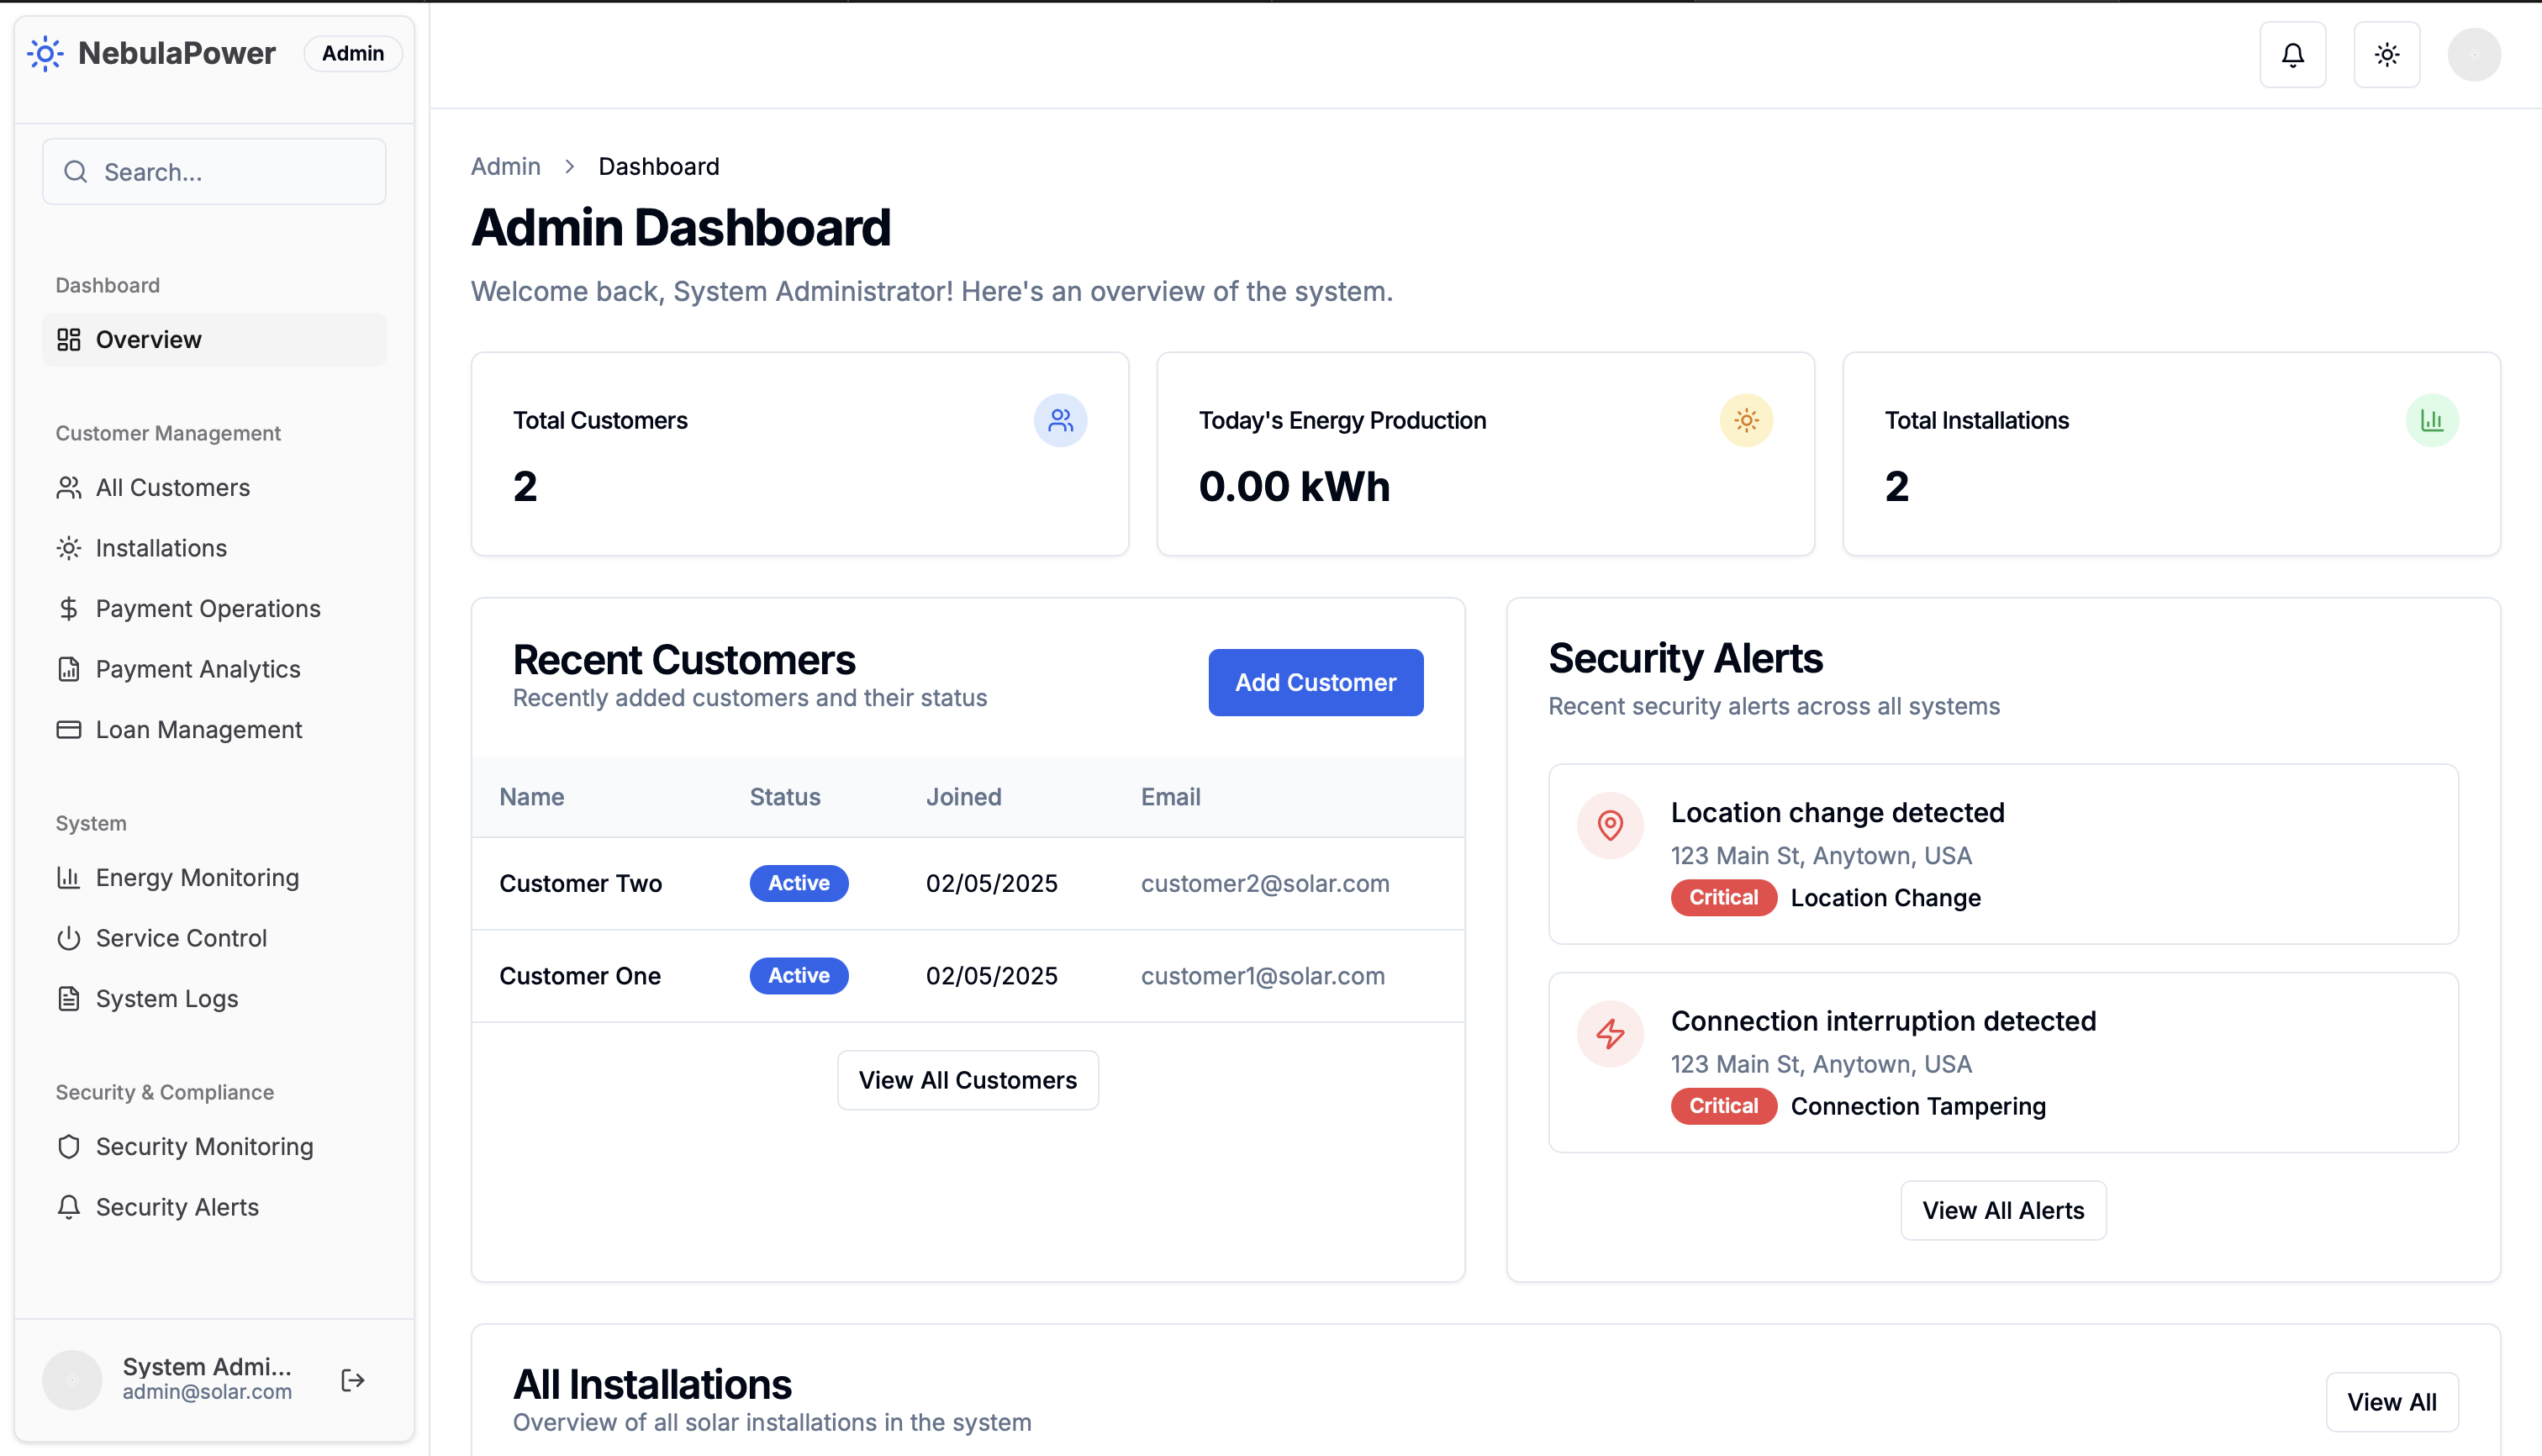
\includegraphics[width=0.9\textwidth]{images_2/admin_dashboard.png}
    \caption{Administrator dashboard}
    \label{fig:admin-dashboard}
\end{figure}

\subsubsection{Customer Dashboard}
\label{subsubsec:customer-dashboard}

Shows installation summary, loan status, payment information, with tabs for Overview, Installations, Payments. See Figure~\ref{fig:customer-dashboard}.

\begin{figure}[h]
    \centering
    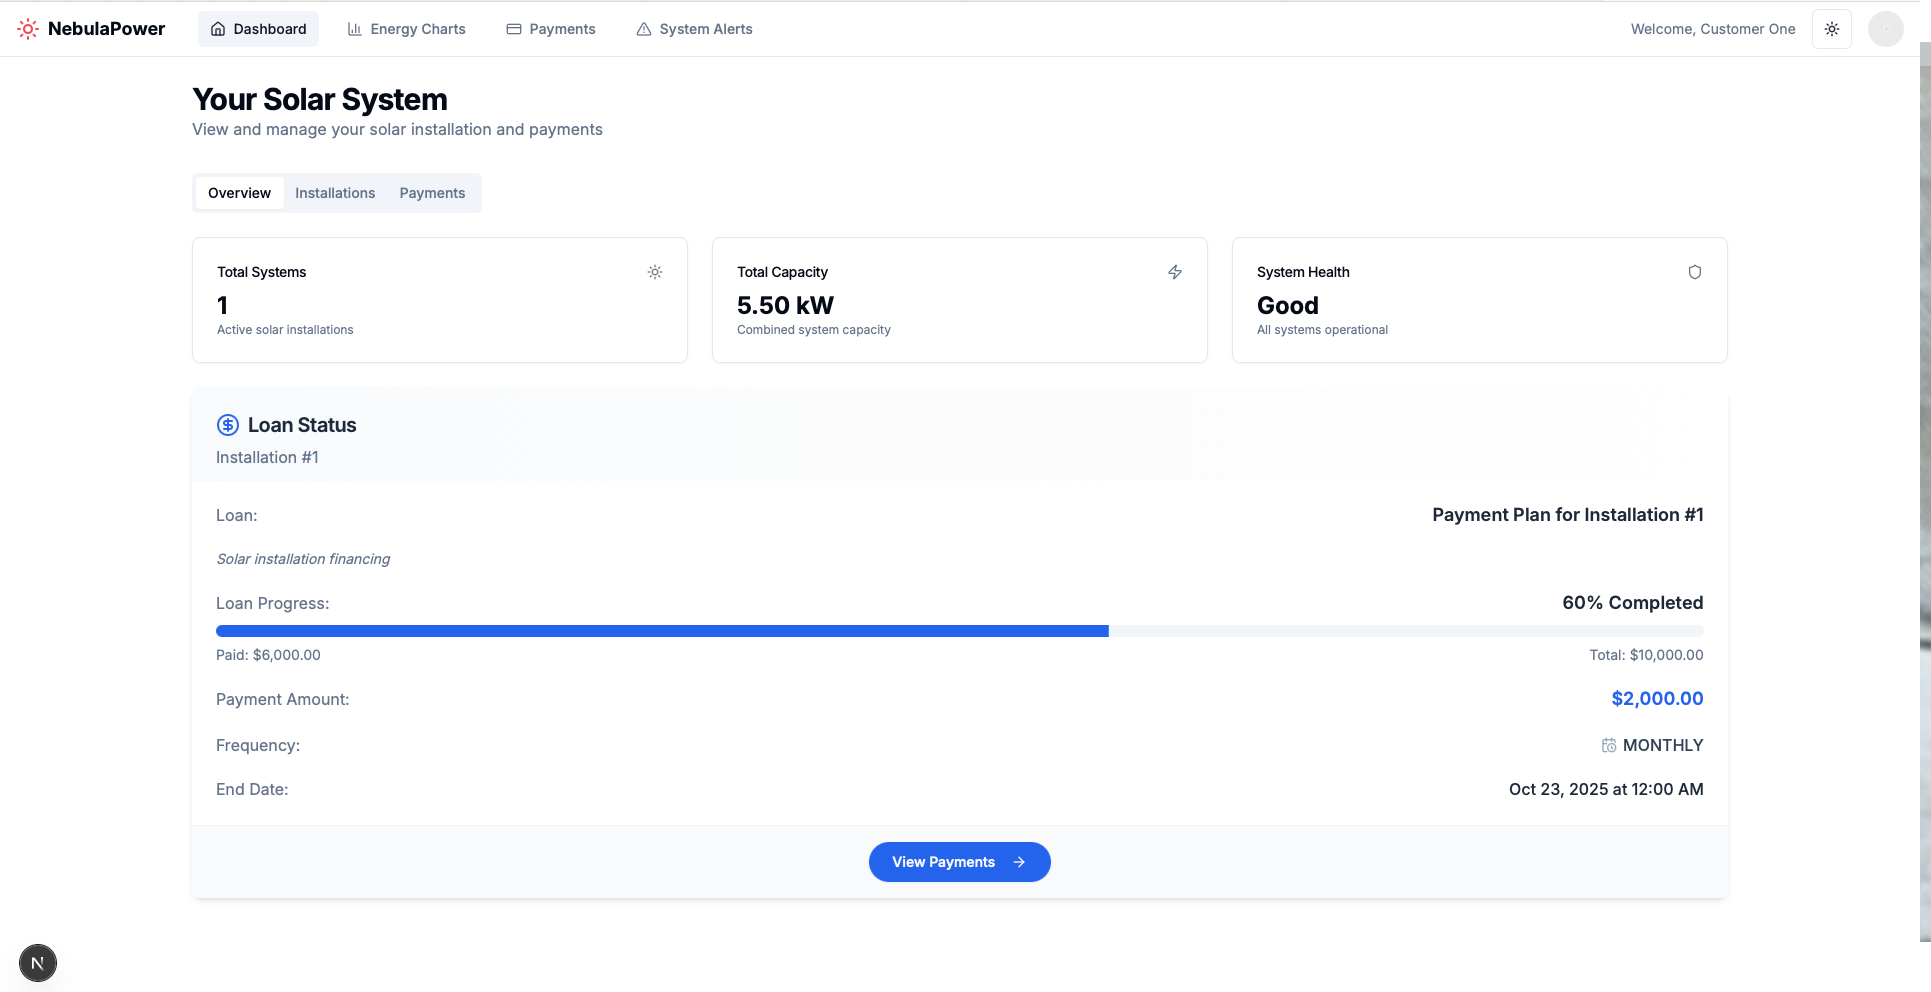
\includegraphics[width=0.9\textwidth]{images_2/customer_dashboard.png}
    \caption{Customer dashboard}
    \label{fig:customer-dashboard}
\end{figure}

\subsection{Energy Monitoring}
\label{subsec:energy-monitoring}

\textbf{Customer View:} Shows current generation, daily/monthly production, efficiency, environmental impact, with production graphs and health indicators (Figure~\ref{fig:customer-energy}).

\begin{figure}[h]
    \centering
    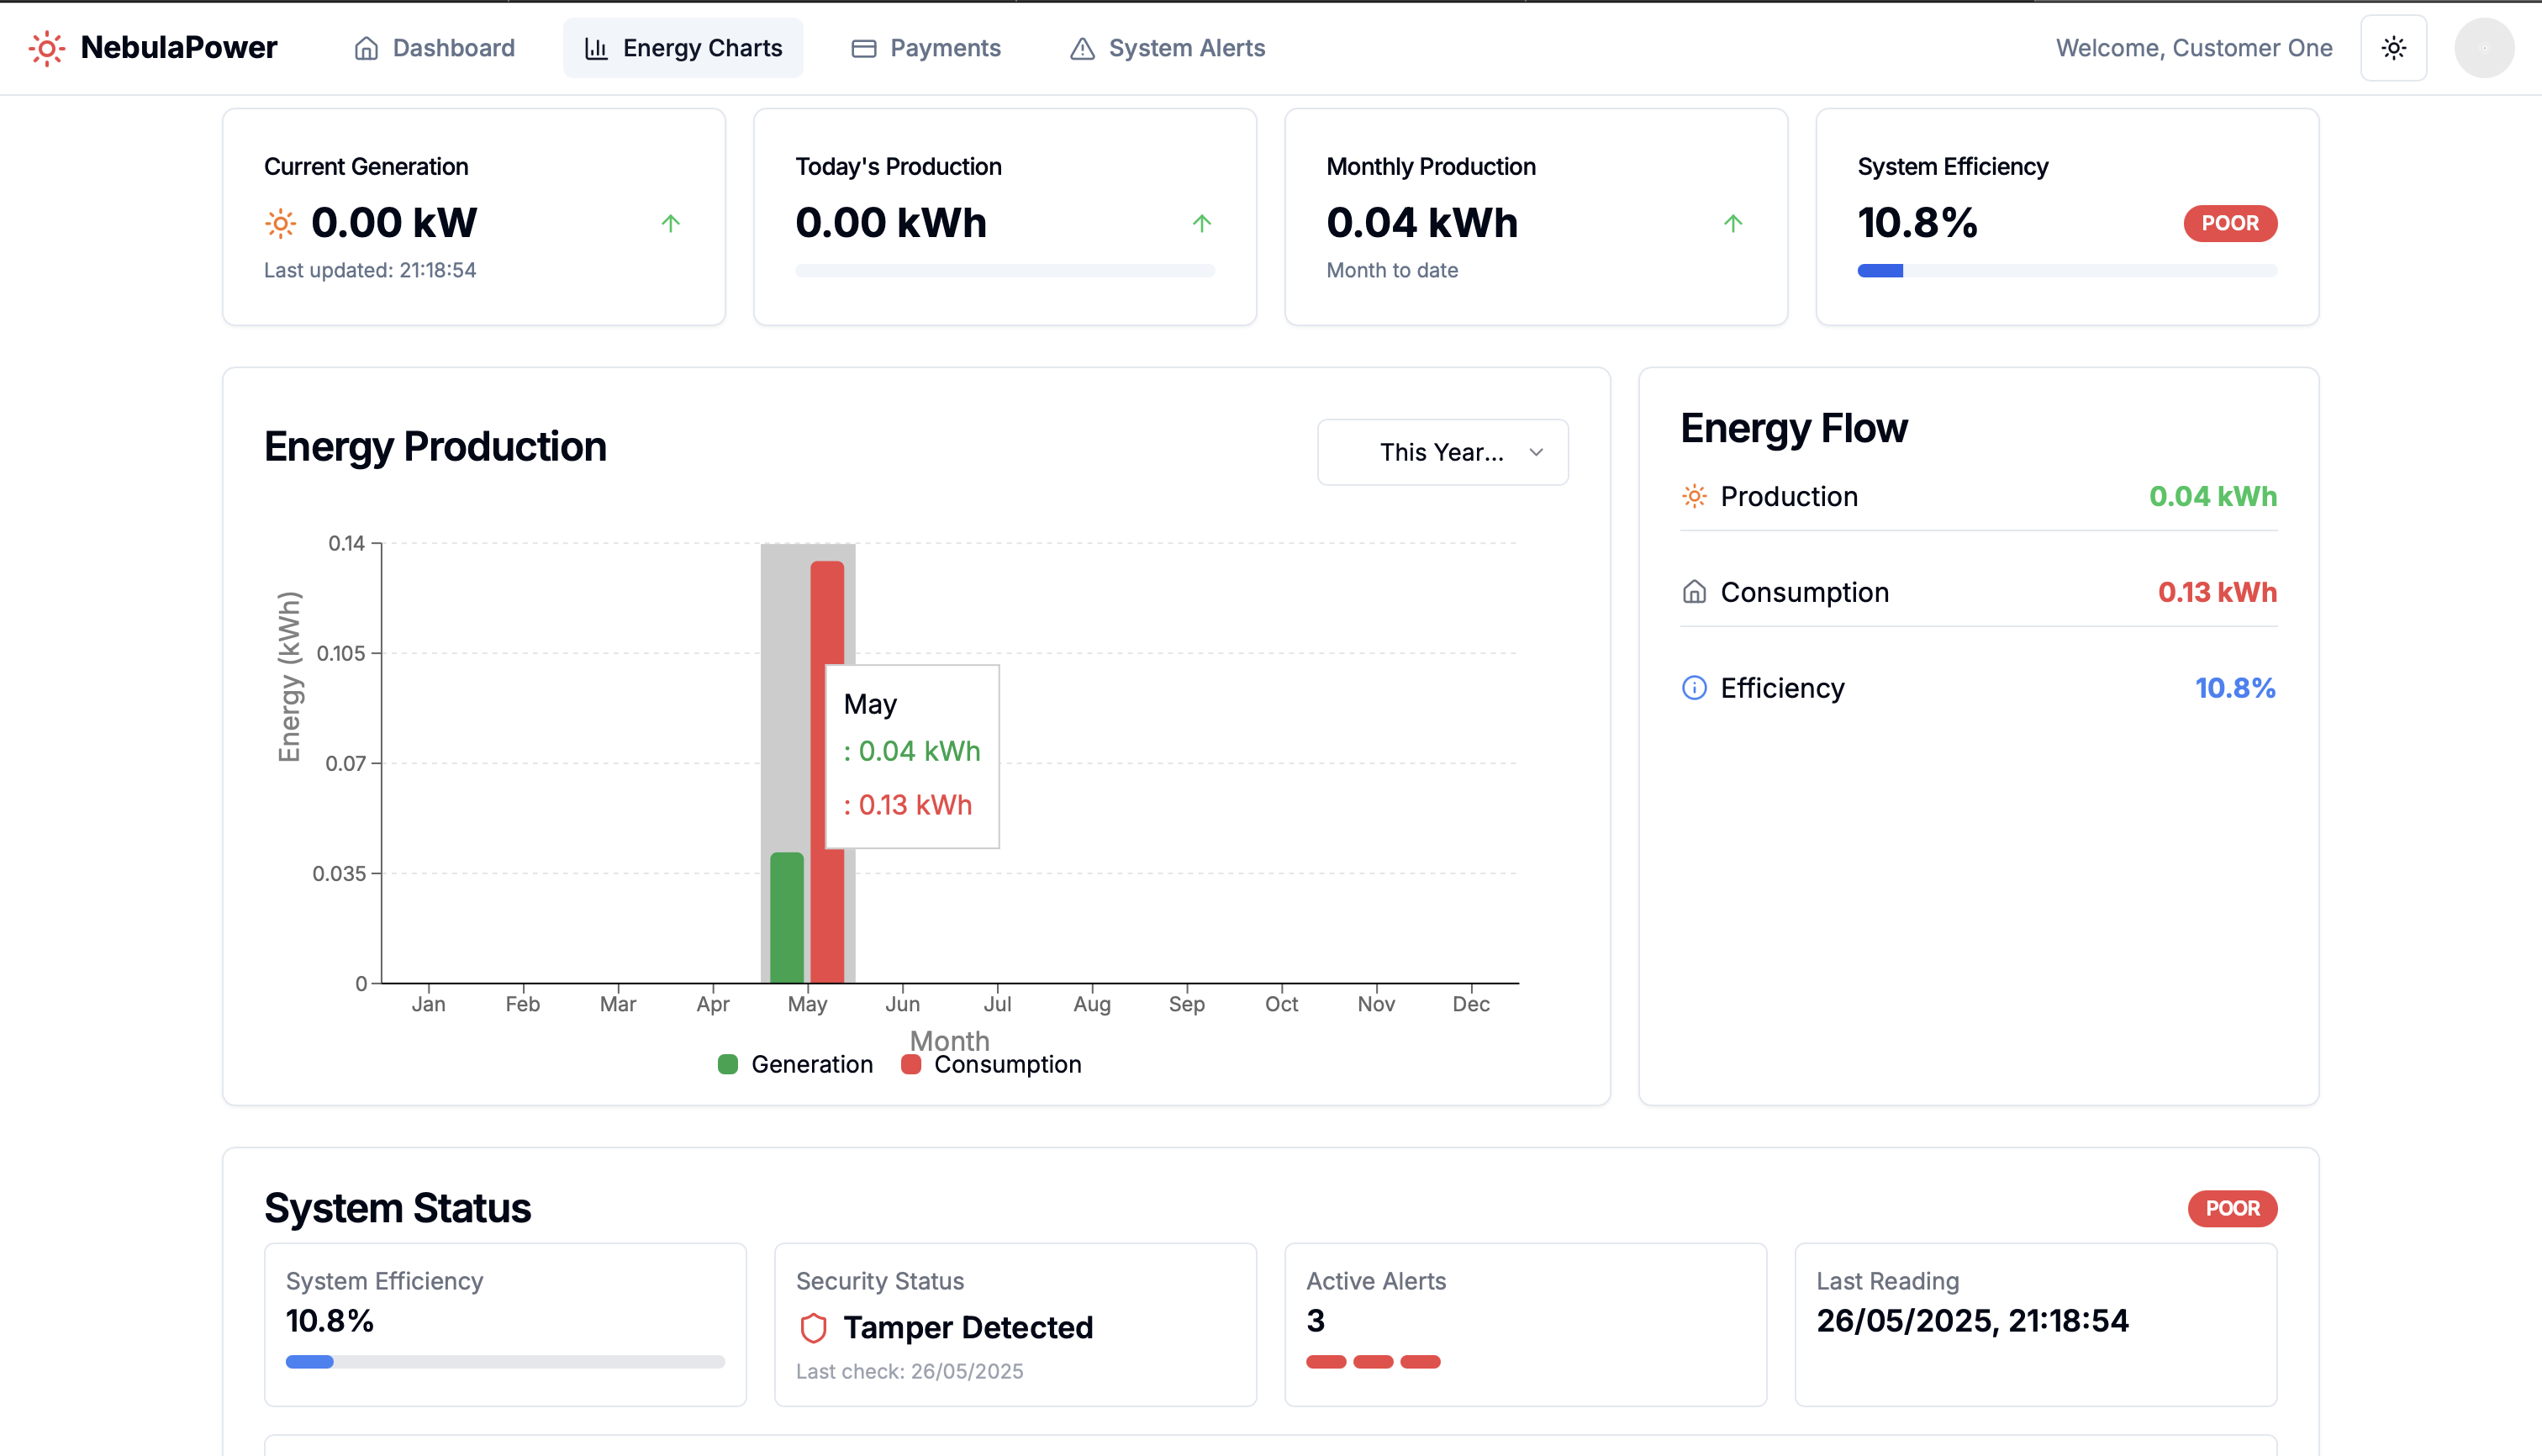
\includegraphics[width=0.85\textwidth]{images_2/customer_energy_dashb.png}
    \caption{Customer energy monitoring dashboard}
    \label{fig:customer-energy}
\end{figure}

\textbf{Admin View:} Displays aggregated metrics, installation comparisons, performance rankings, status indicators across all systems (Figure~\ref{fig:admin-energy}).

\begin{figure}[h]
    \centering
    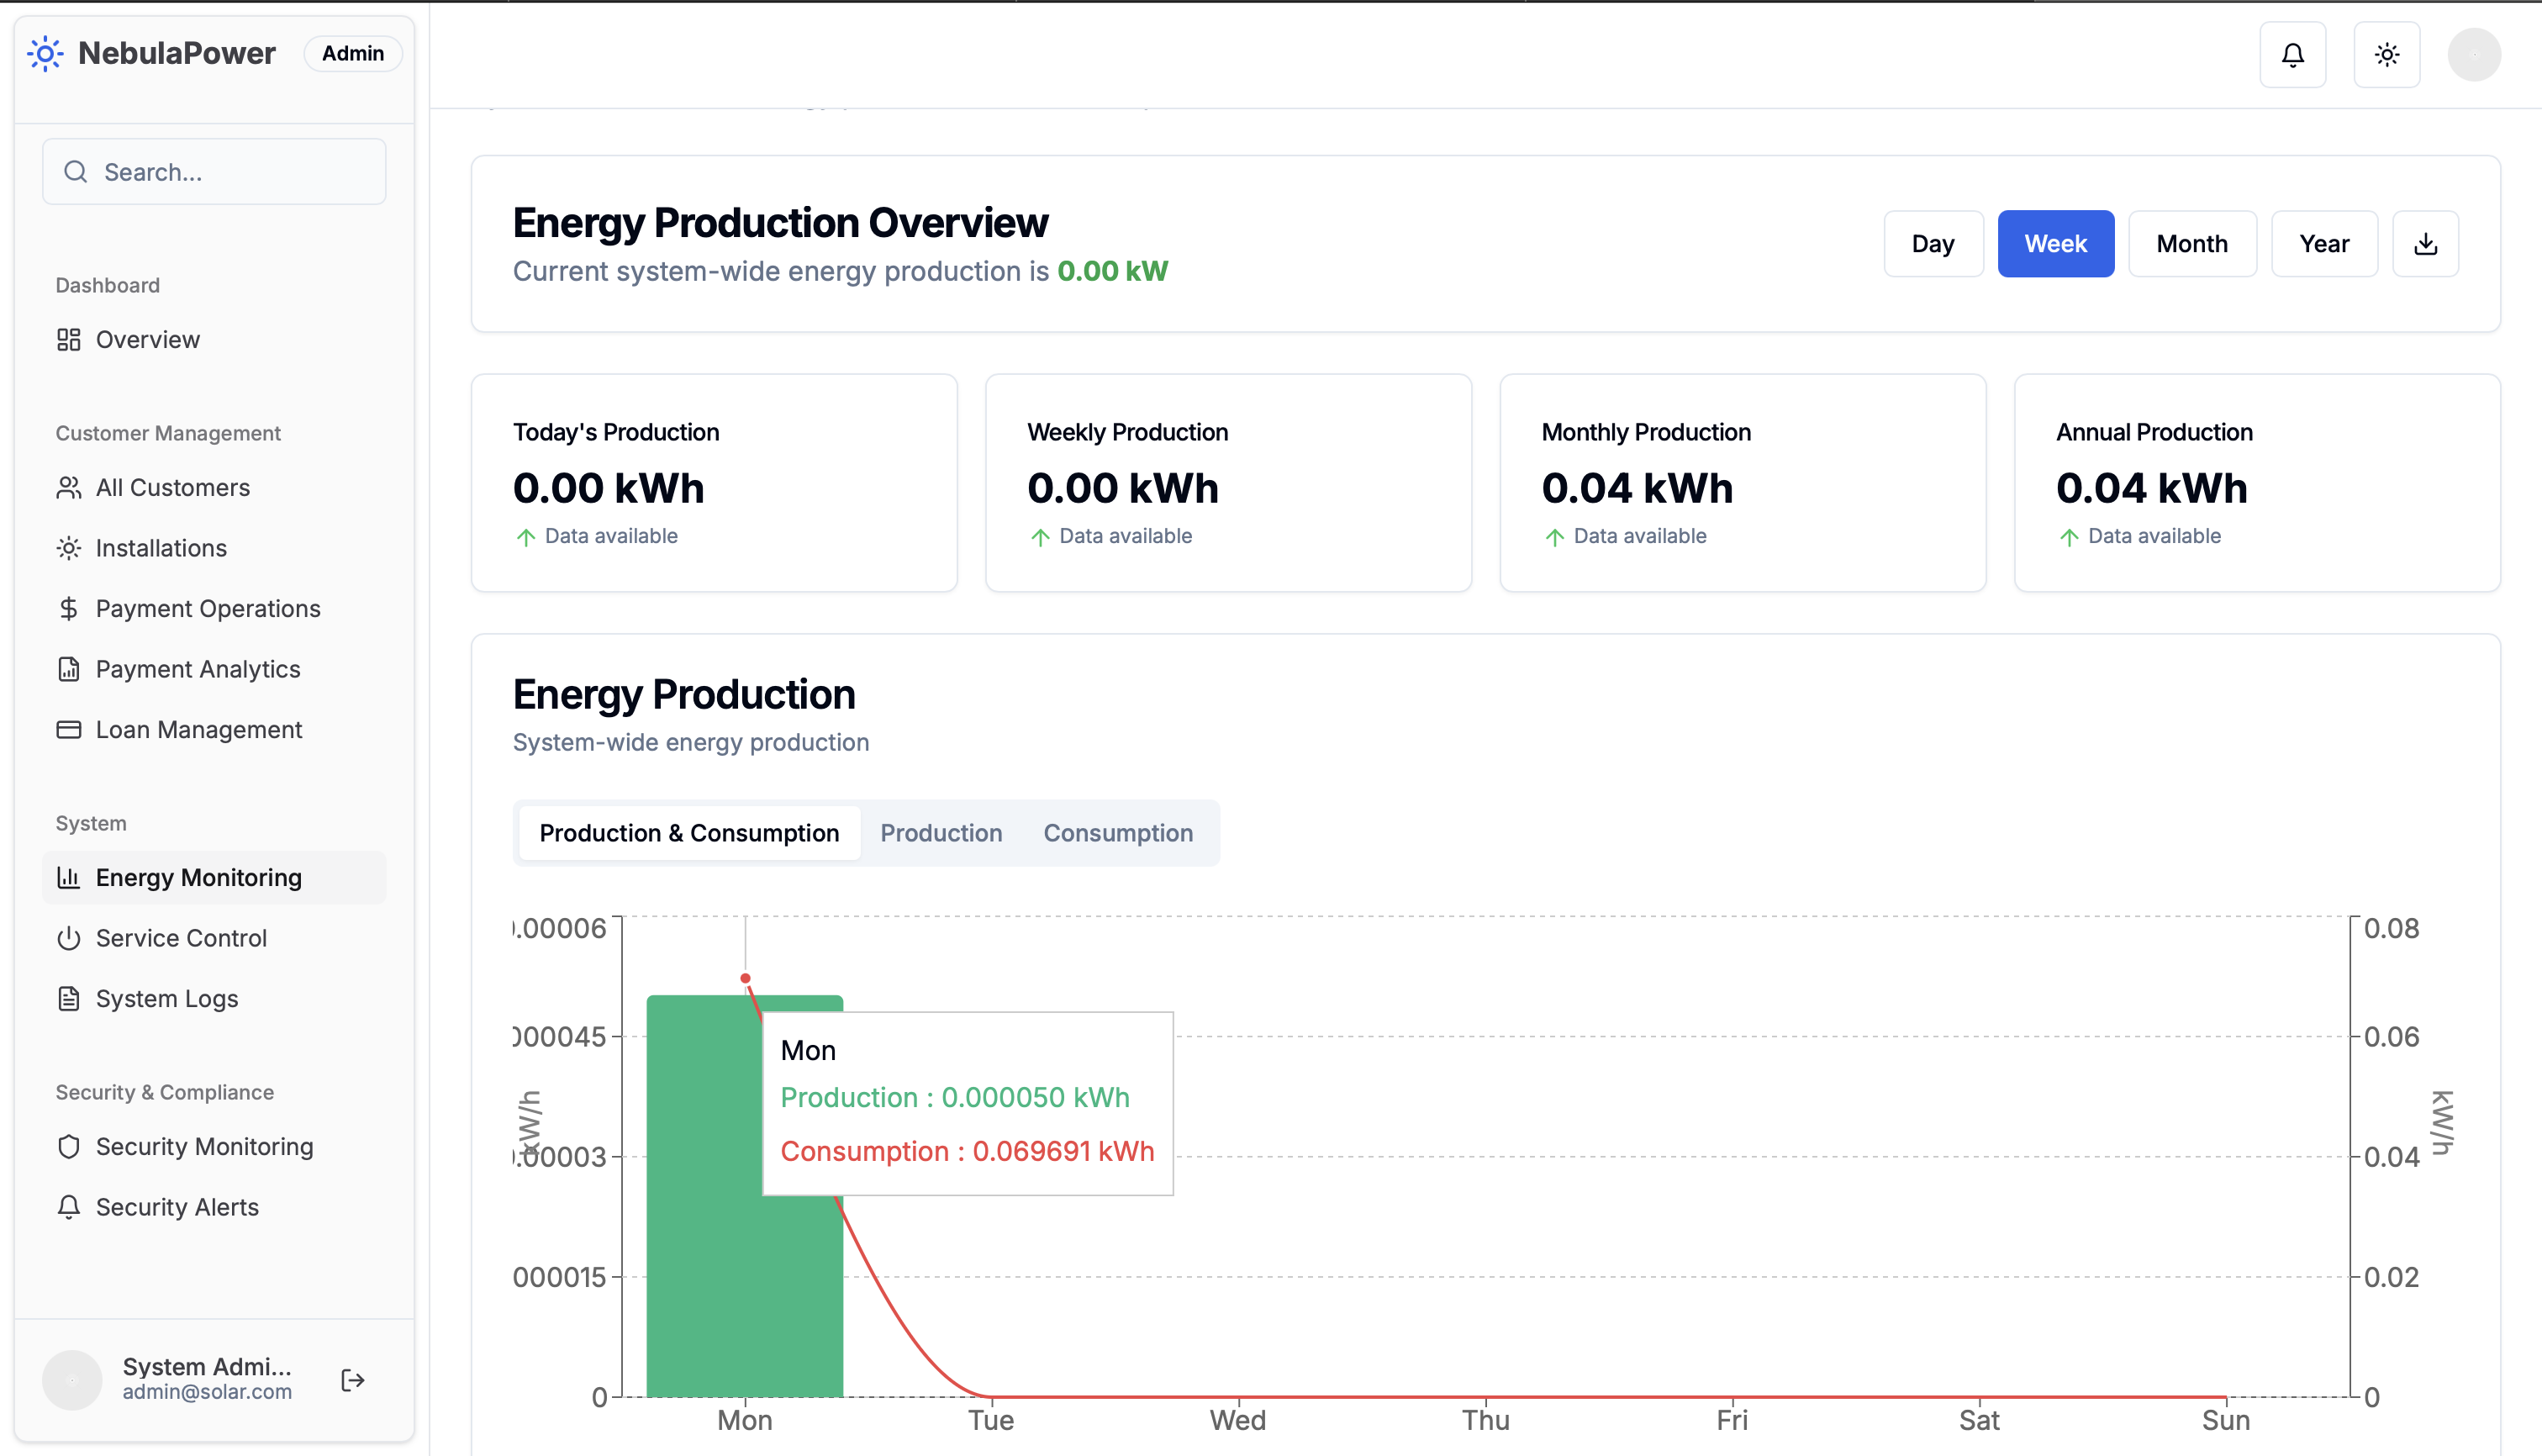
\includegraphics[width=0.85\textwidth]{images_2/admin_energy_dashb.png}
    \caption{Administrator energy monitoring}
    \label{fig:admin-energy}
\end{figure}

\subsection{Payment Operations Interface}
\label{subsec:payment-interface}

\textbf{Admin Views:} Payment analytics (trends, status tracking, Figure~\ref{fig:payment-analytics}), loan management (configuration, assignments, Figure~\ref{fig:payment-plans}), payment history (transactions, reconciliation, Figure~\ref{fig:payment-history}).

\begin{figure}[h]
    \centering
    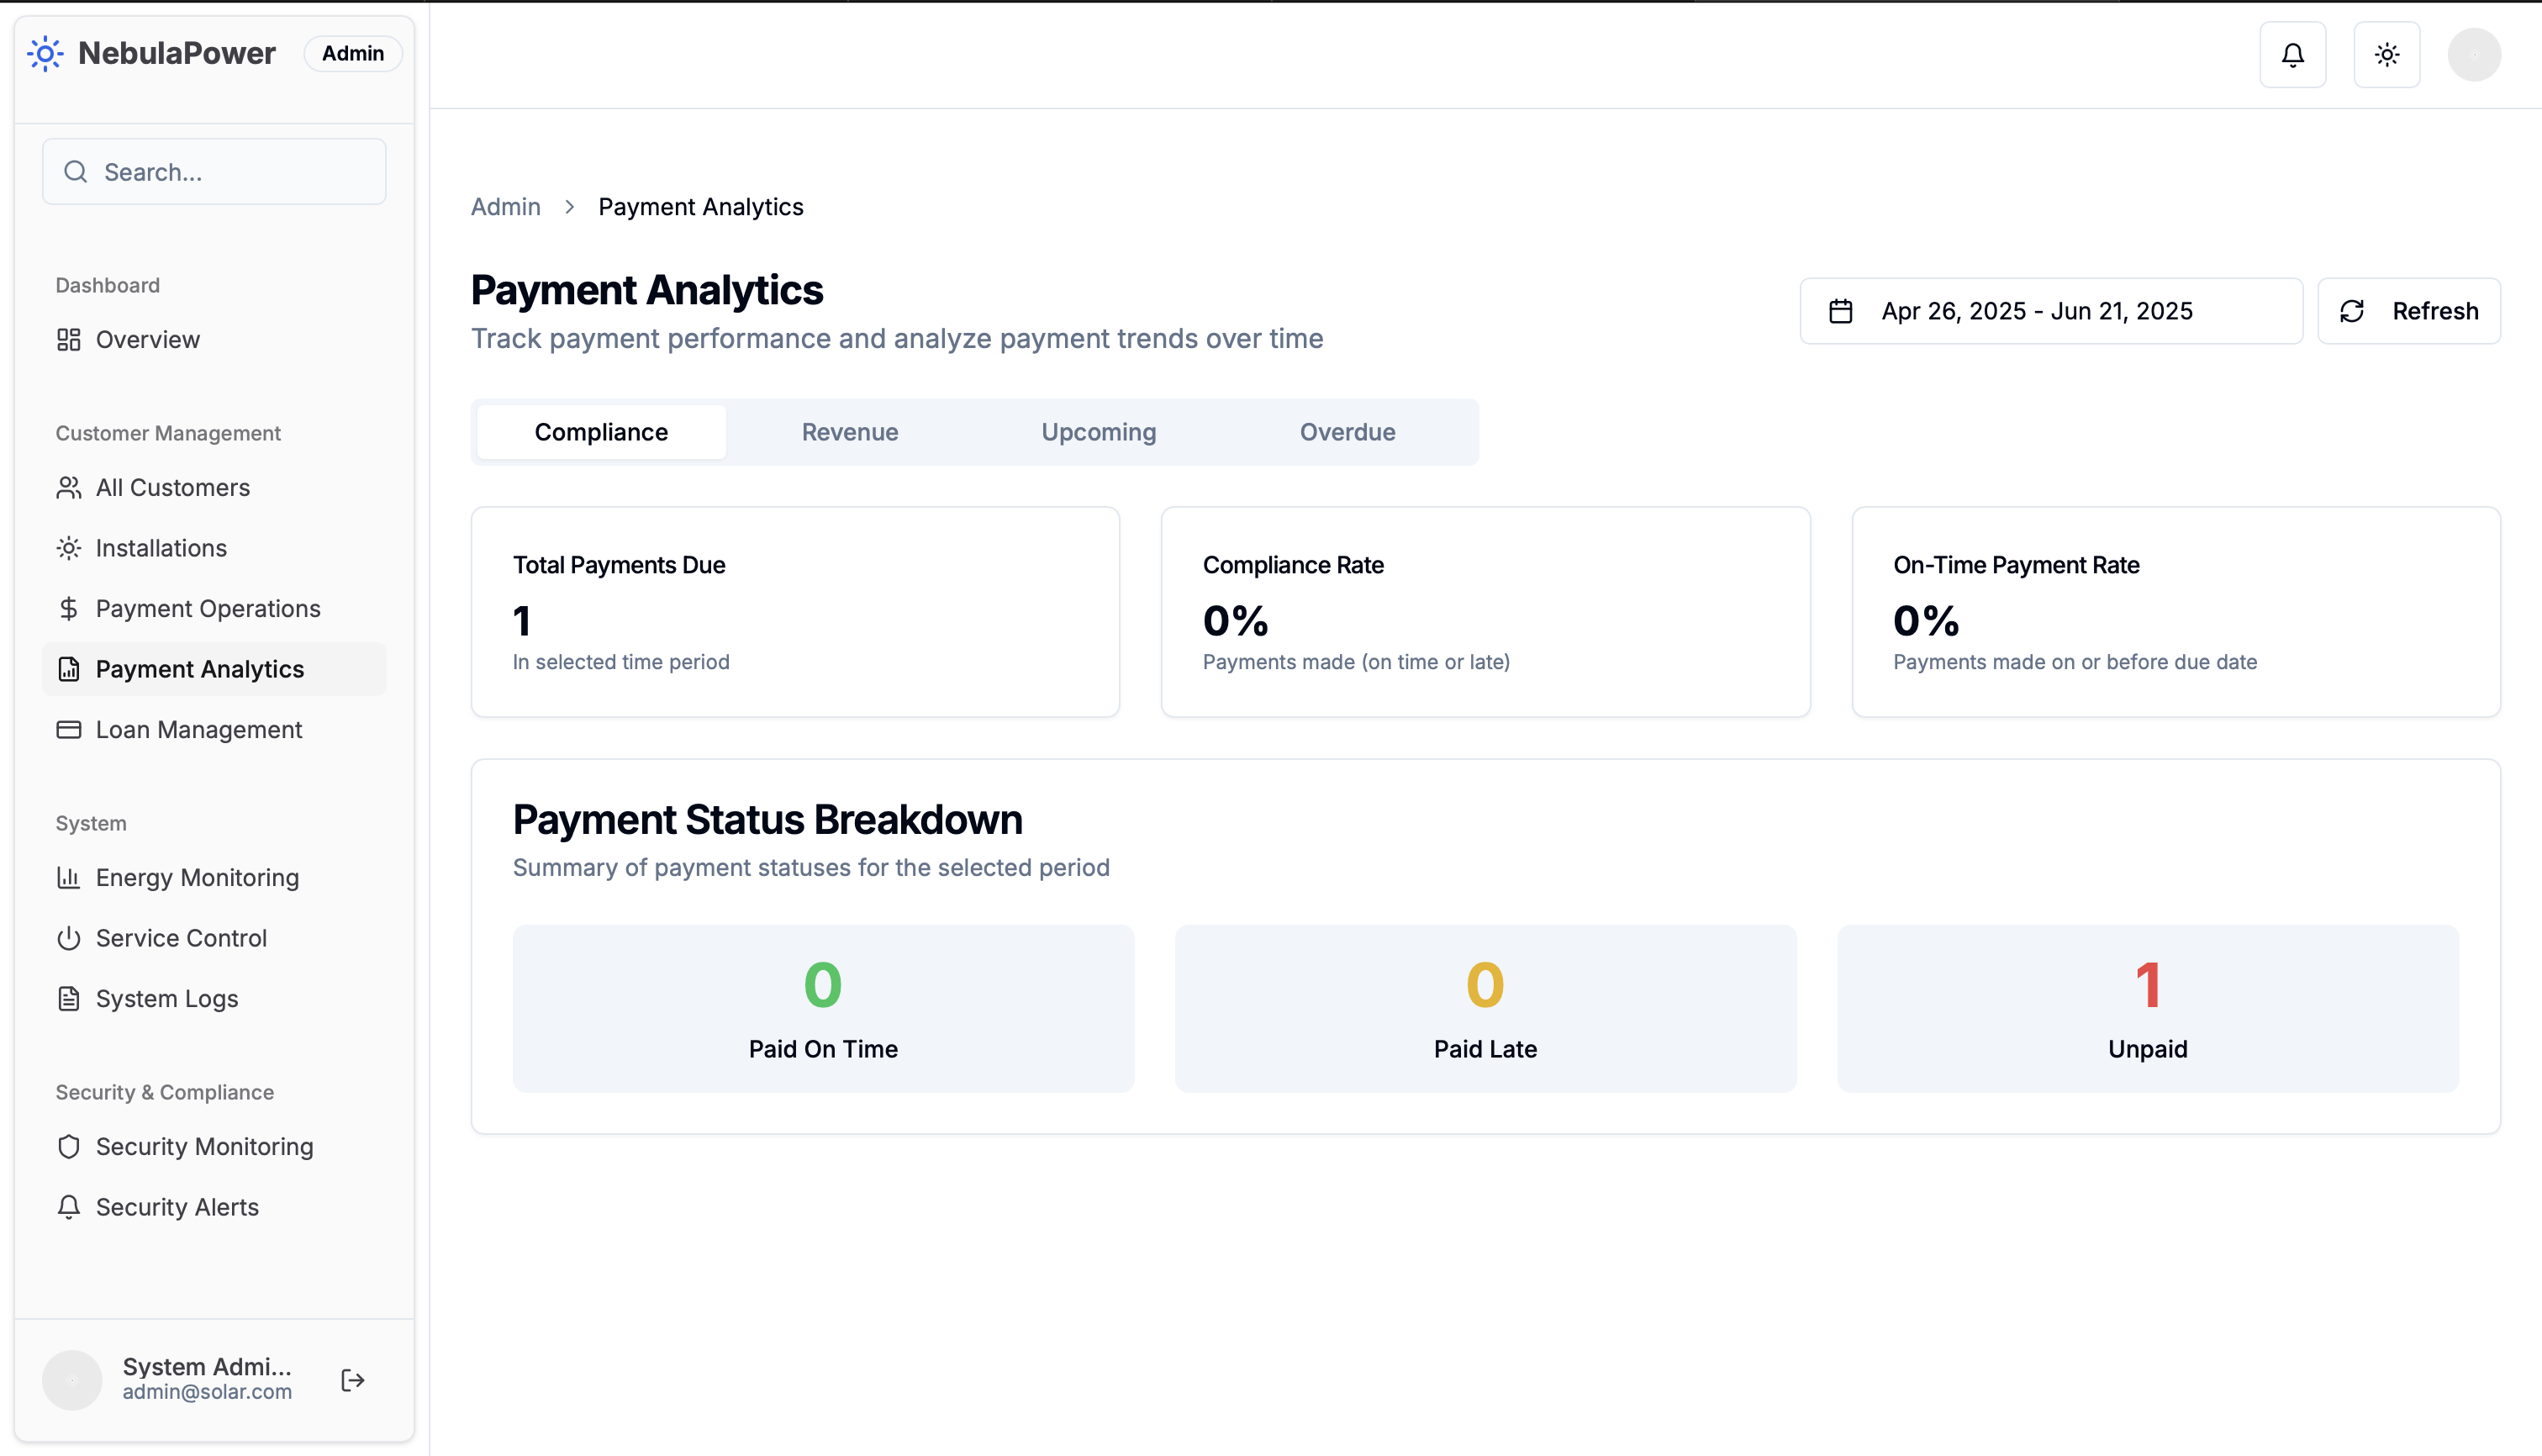
\includegraphics[width=0.85\textwidth]{images_2/payment_analytics.png}
    \caption{Payment analytics}
    \label{fig:payment-analytics}
\end{figure}

\begin{figure}[h]
    \centering
    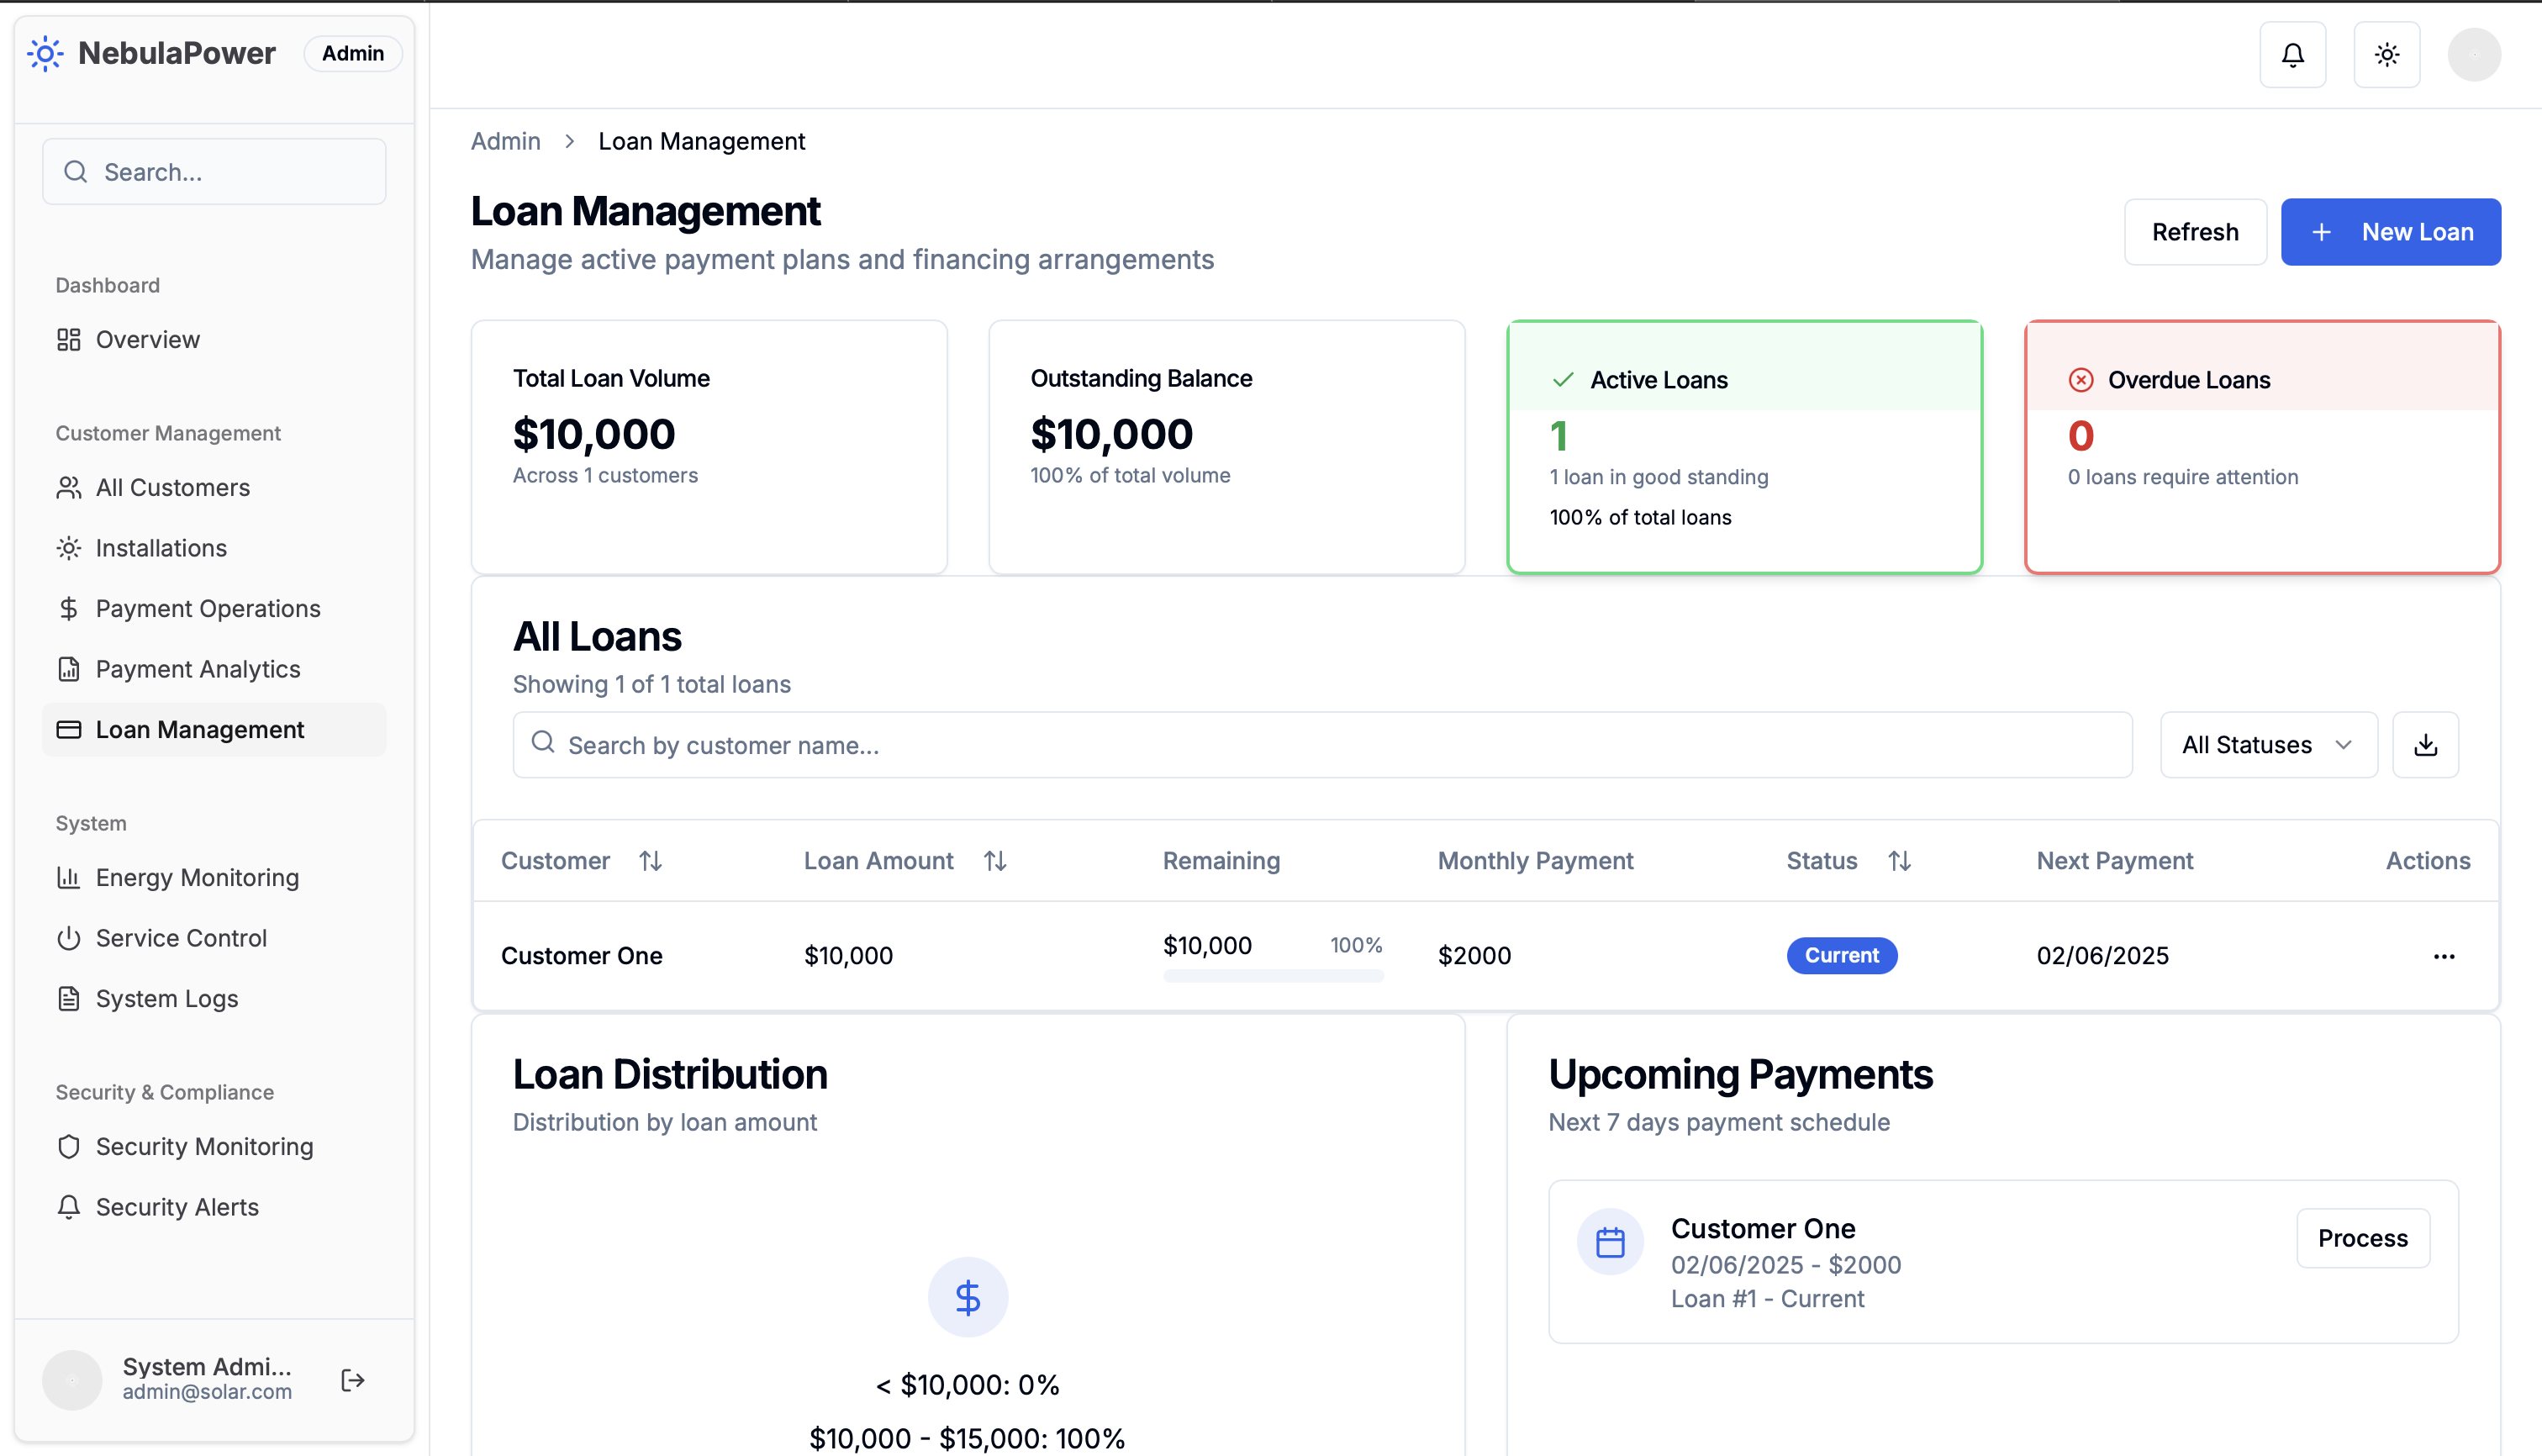
\includegraphics[width=0.85\textwidth]{images_2/loan_management.png}
    \caption{Loan management}
    \label{fig:payment-plans}
\end{figure}

\begin{figure}[h]
    \centering
    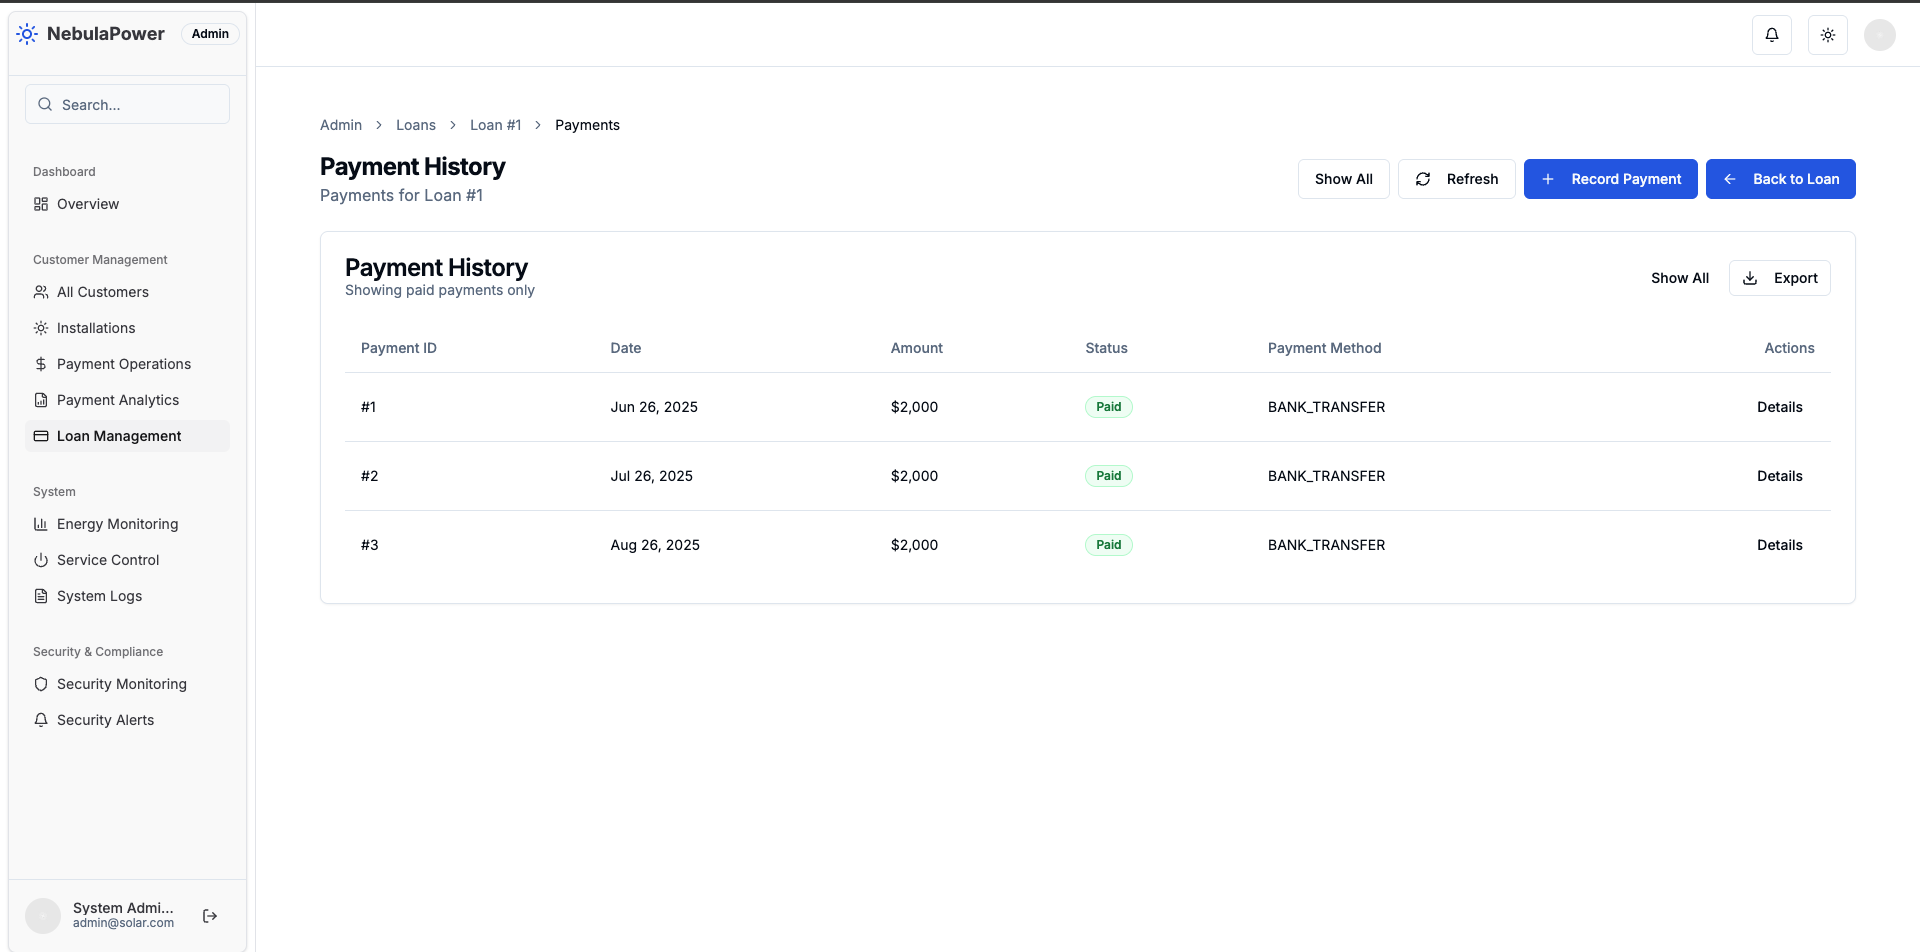
\includegraphics[width=0.85\textwidth]{images_2/admin_payment_history.png}
    \caption{Payment history}
    \label{fig:payment-history}
\end{figure}

\textbf{Customer View:} Loan summary, payment schedule, progress tracking, transaction history (Figure~\ref{fig:customer-payment-view}).

\begin{figure}[h]
    \centering
    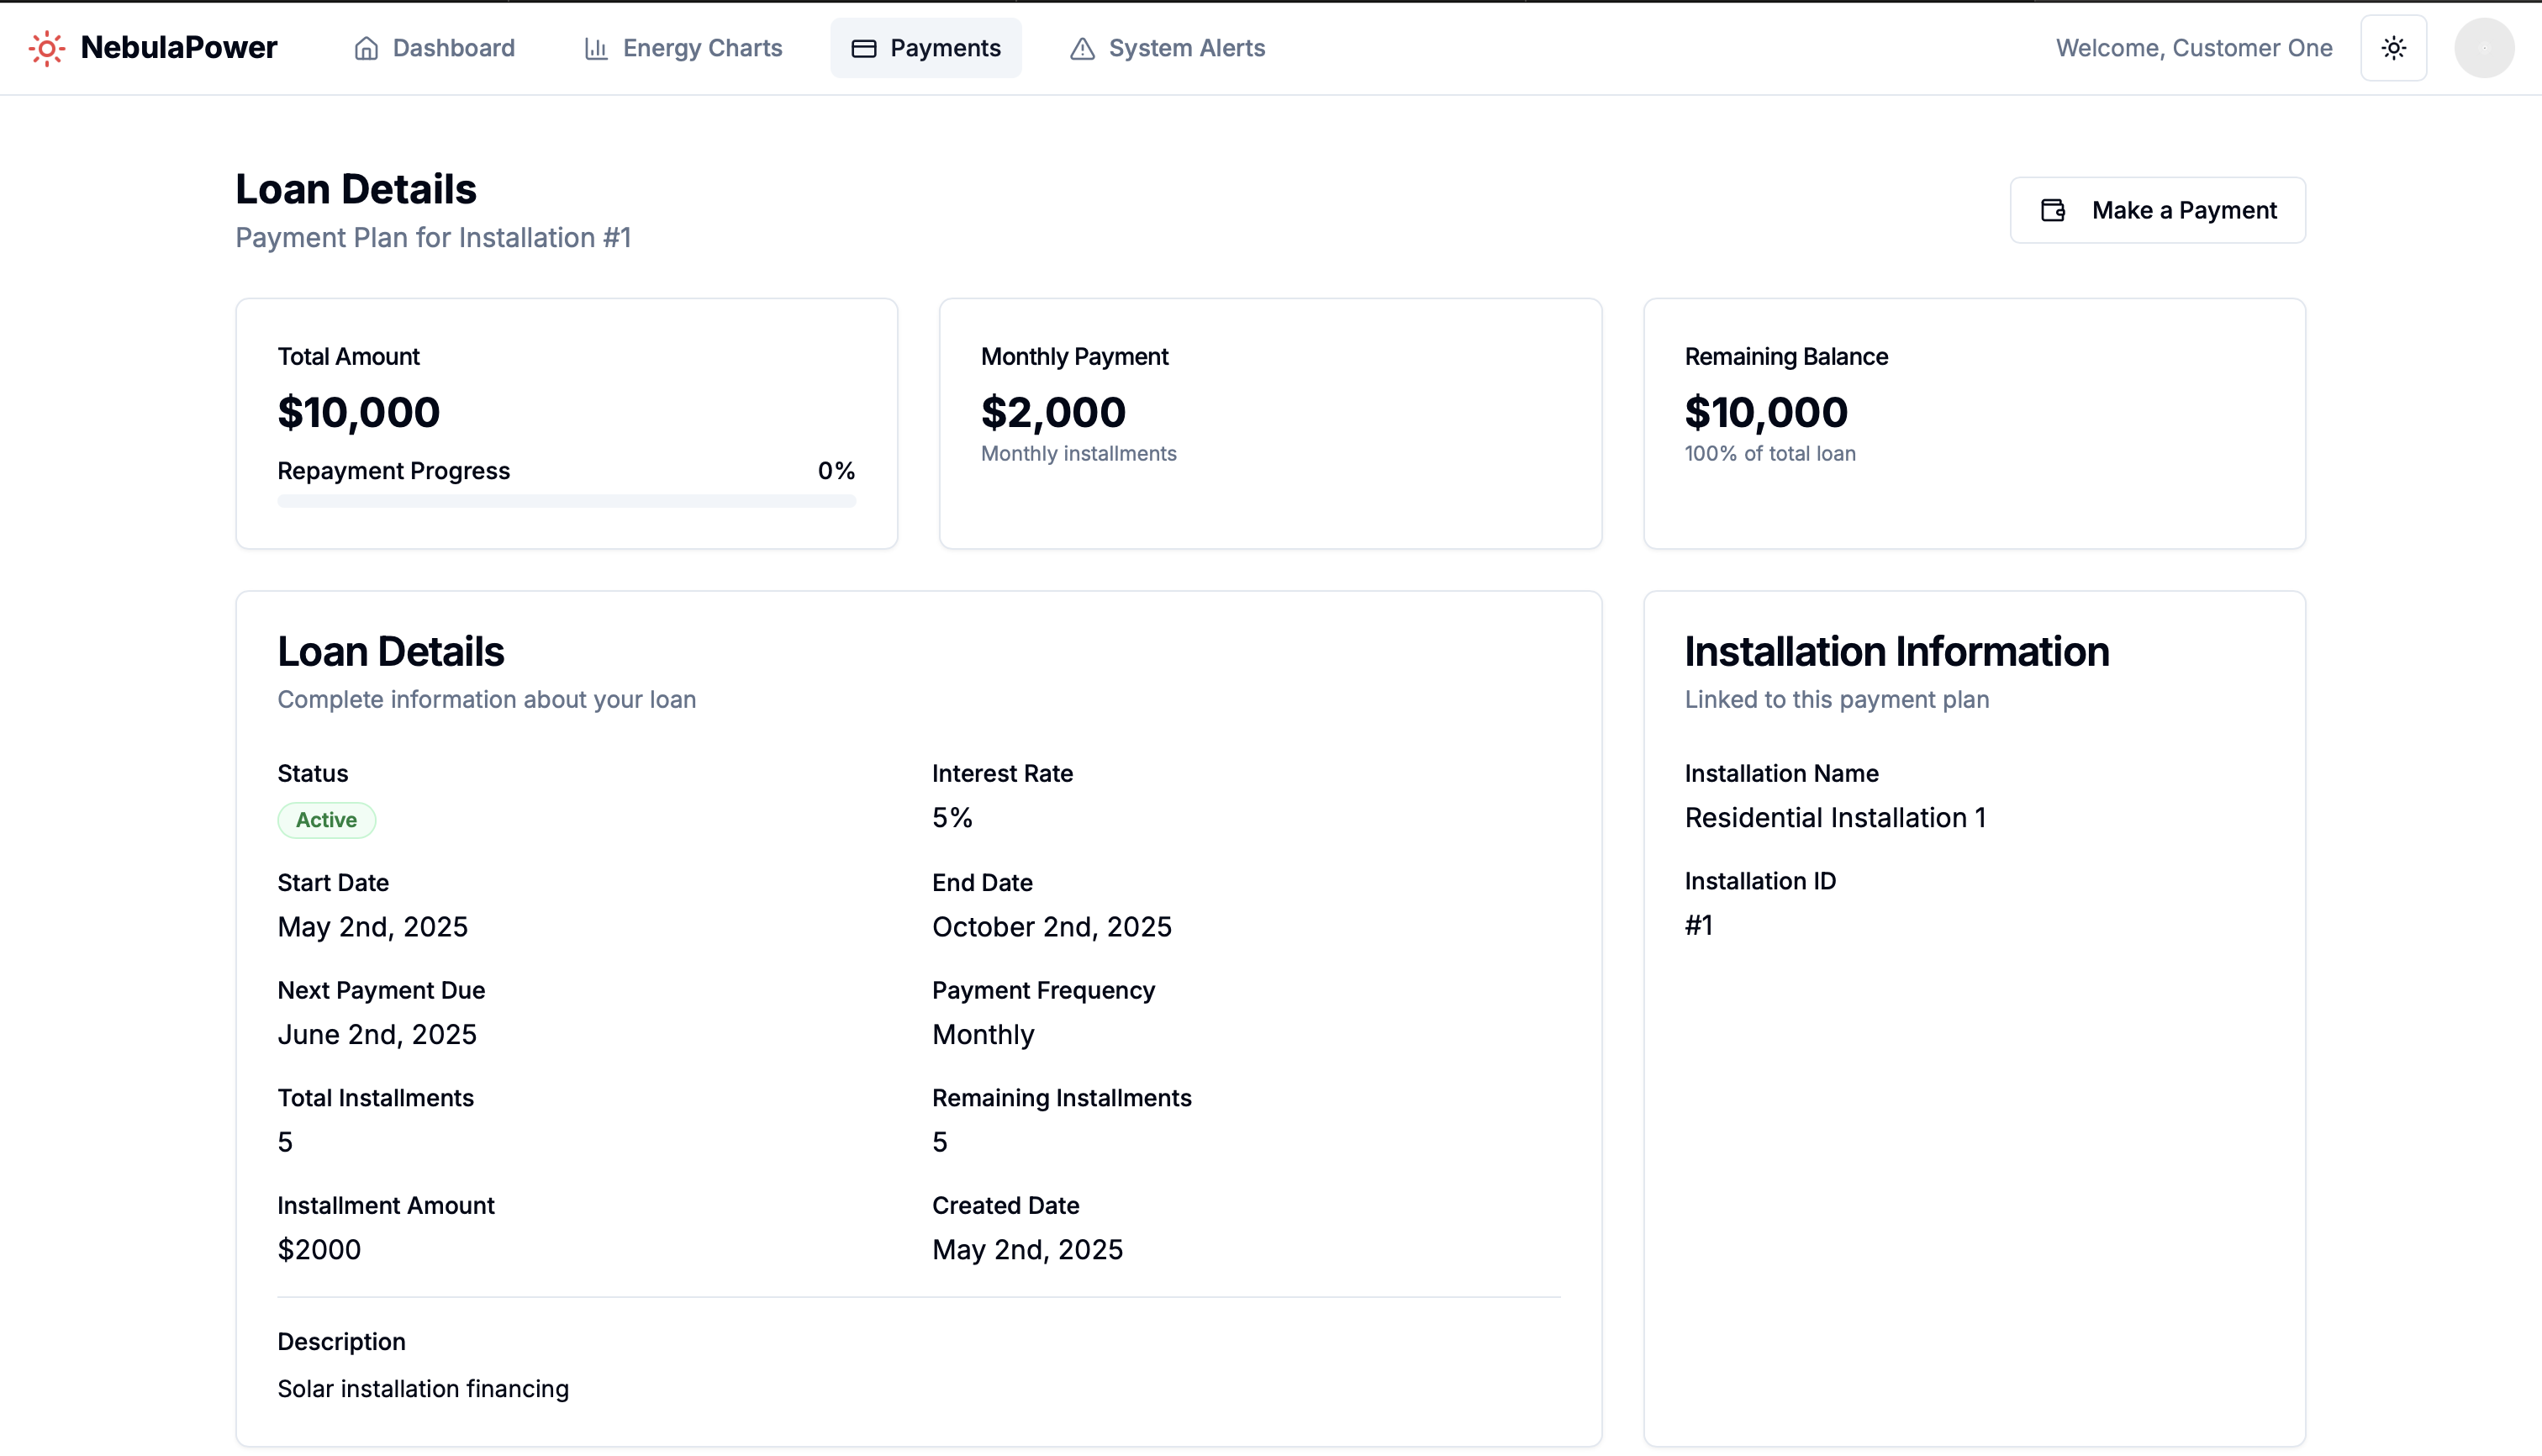
\includegraphics[width=0.85\textwidth]{images_2/customer_payments_view.png}
    \caption{Customer payment view}
    \label{fig:customer-payment-view}
\end{figure}

\subsection{Security \& Compliance Interface}
\label{subsec:security-interface}

\textbf{Security Monitoring:} Access logs, authentication status, health indicators, configuration (Figure~\ref{fig:security-monitoring}).

\begin{figure}[h]
    \centering
    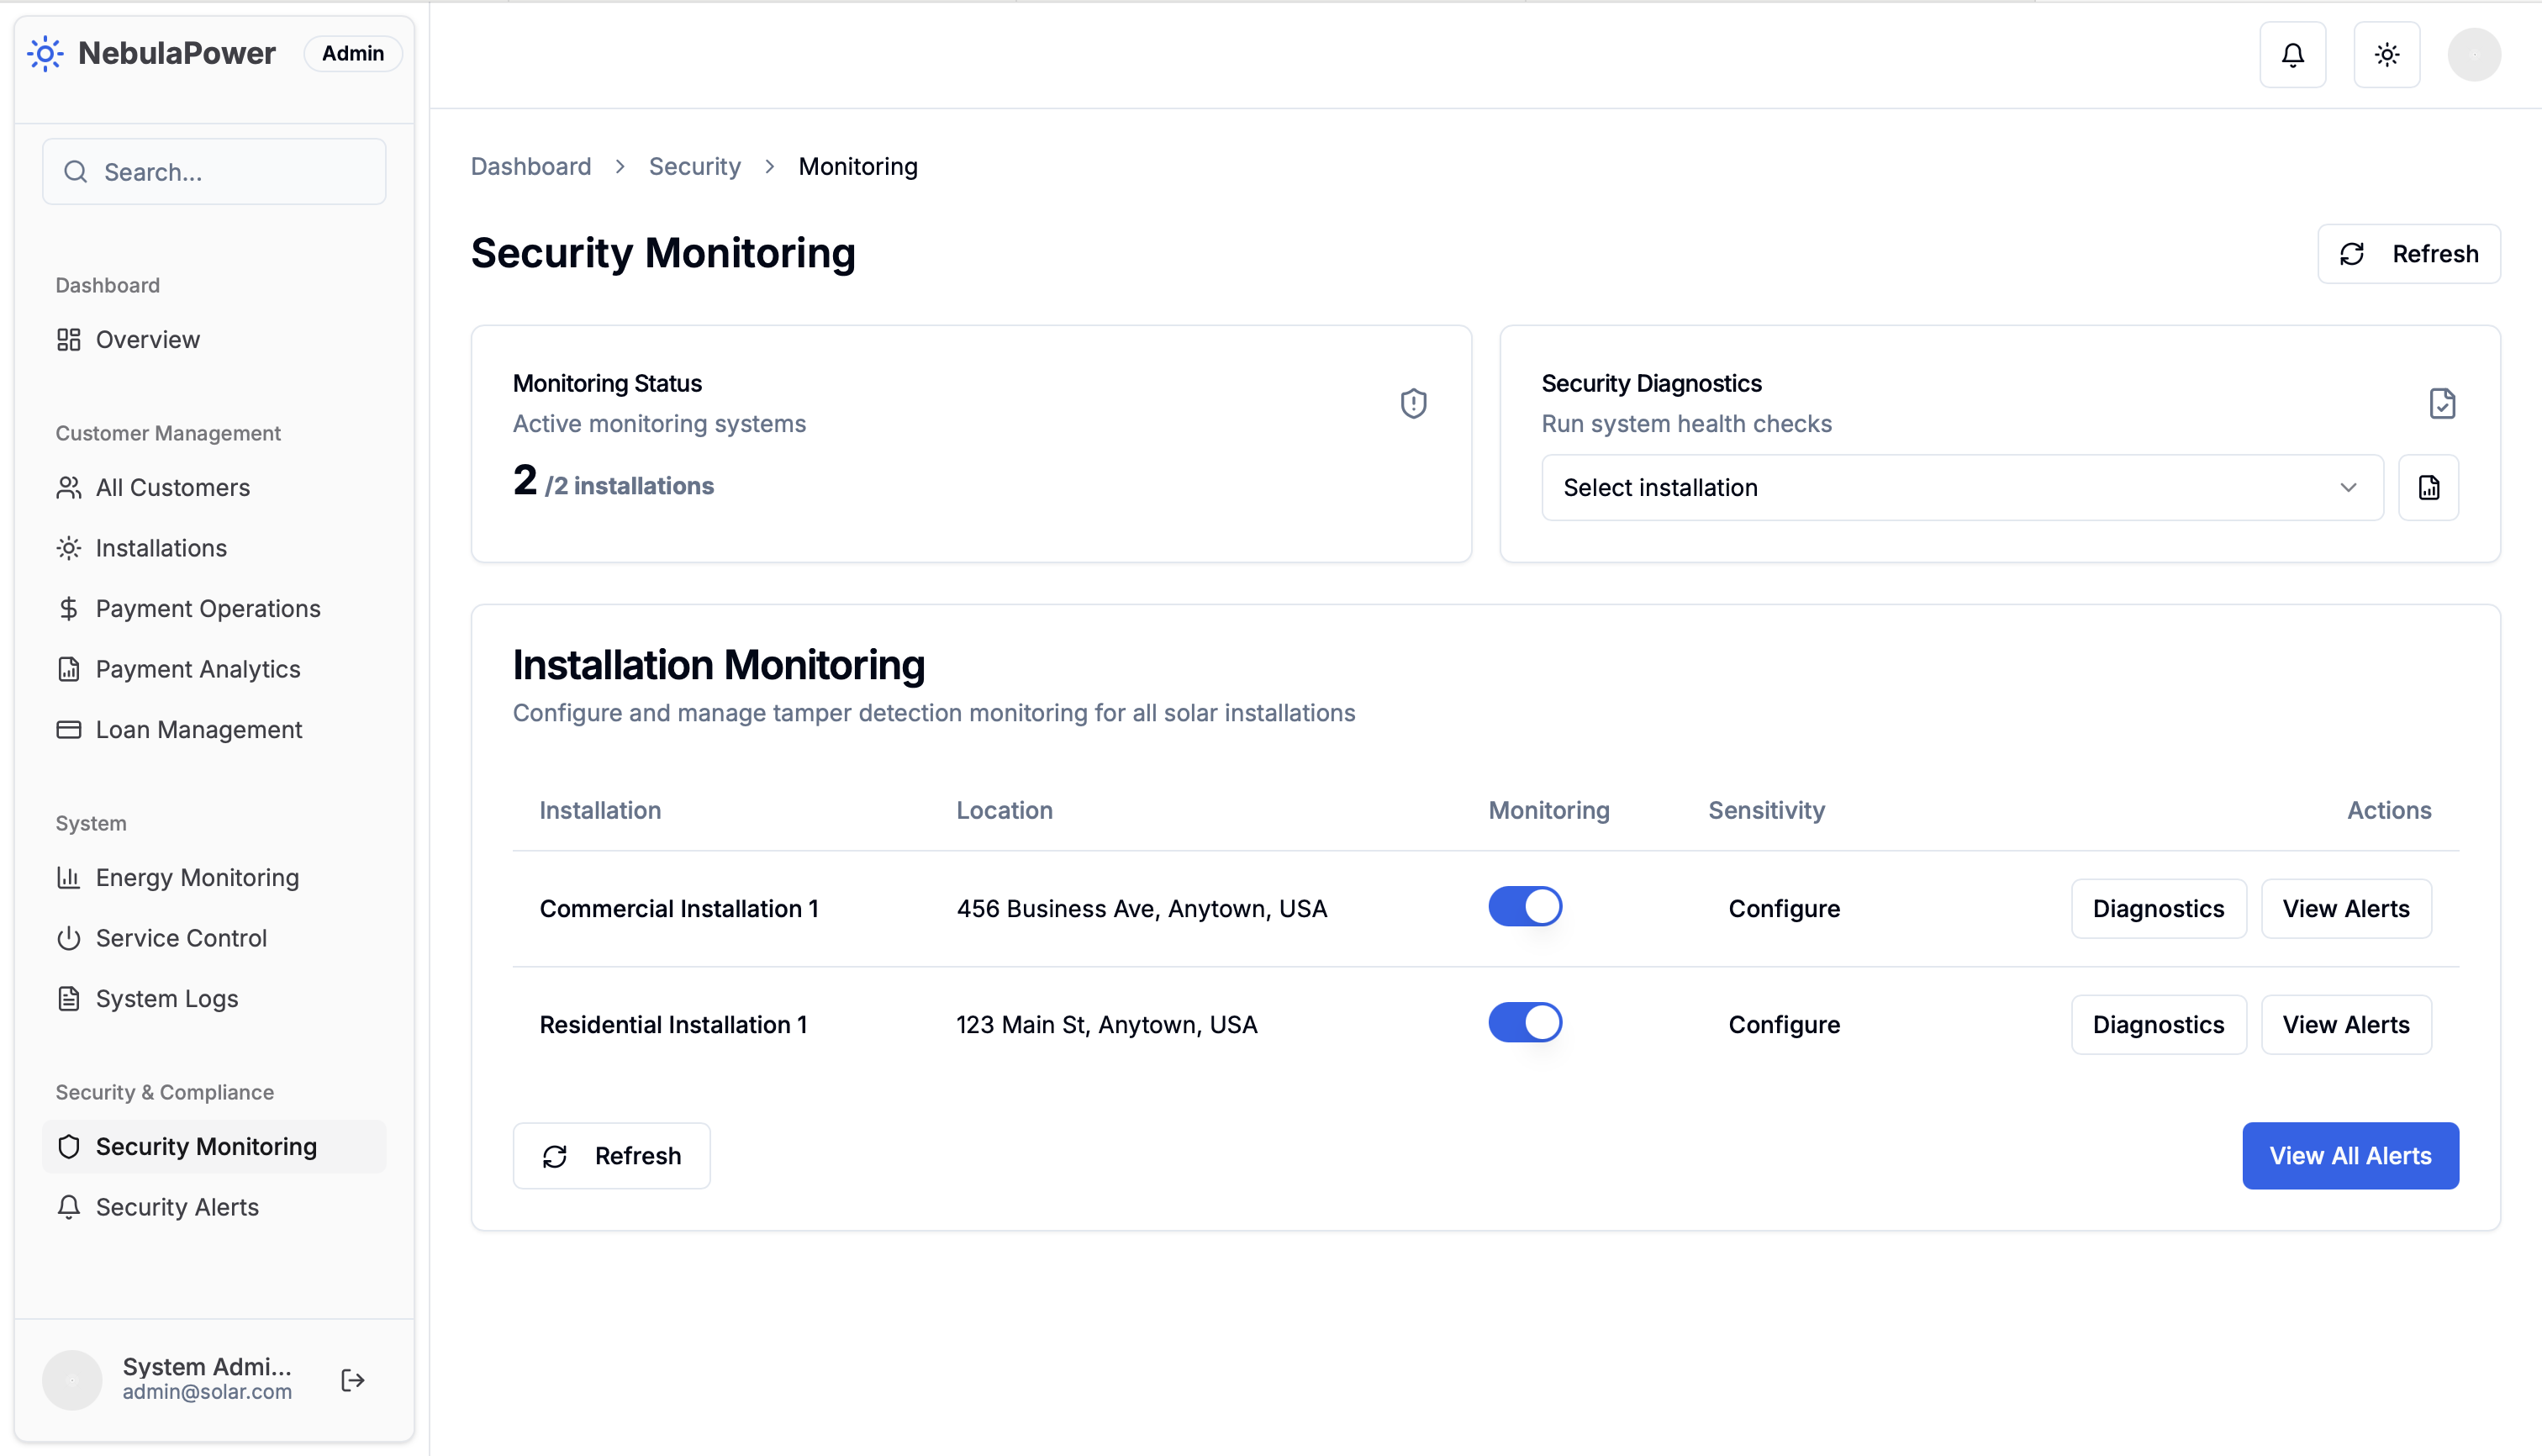
\includegraphics[width=0.85\textwidth]{images_2/admin_security_monitoring.png}
    \caption{Security monitoring}
    \label{fig:security-monitoring}
\end{figure}

\textbf{Admin Alerts:} Dashboard with alert counts, filtering (open/closed/in-progress), severity classification, response actions (Figure~\ref{fig:security-alerts-admin}).

\begin{figure}[h]
    \centering
    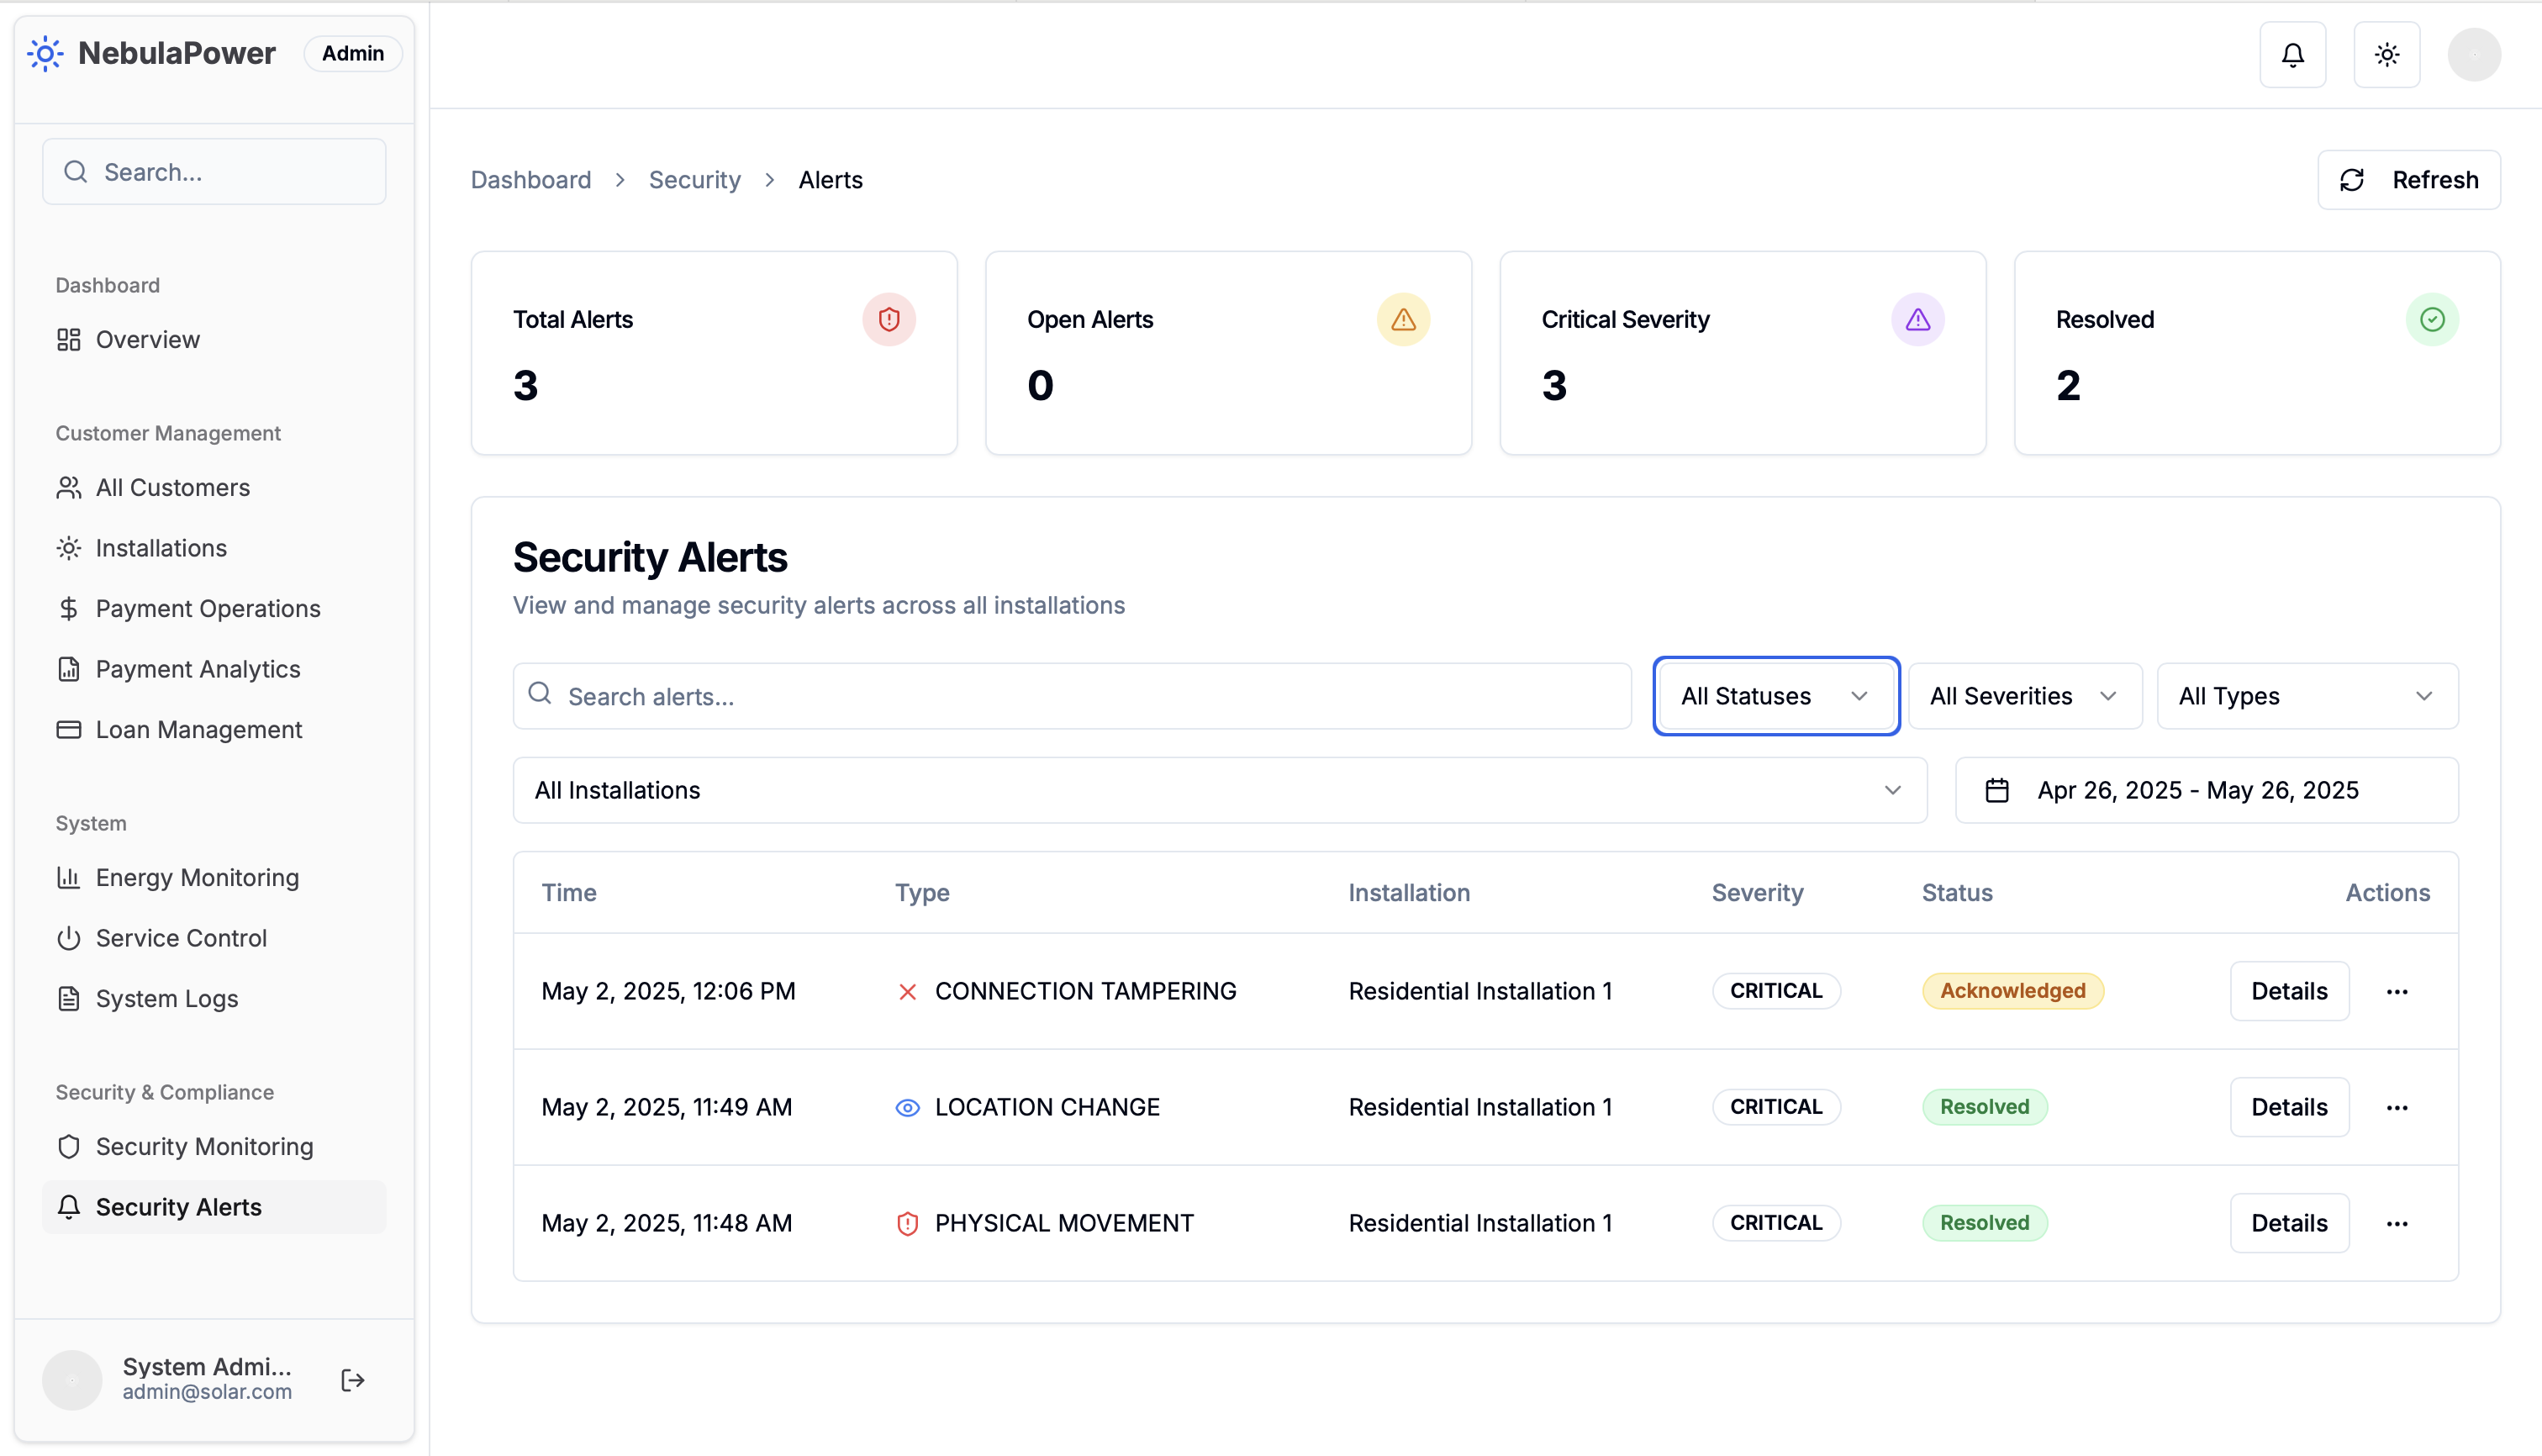
\includegraphics[width=0.85\textwidth]{images_2/admin_alerts.png}
    \caption{Admin security alerts}
    \label{fig:security-alerts-admin}
\end{figure}

\textbf{Customer Alerts:} Installation-specific alerts with status and recommended actions (Figure~\ref{fig:security-alerts-customer}).

\begin{figure}[h]
    \centering
    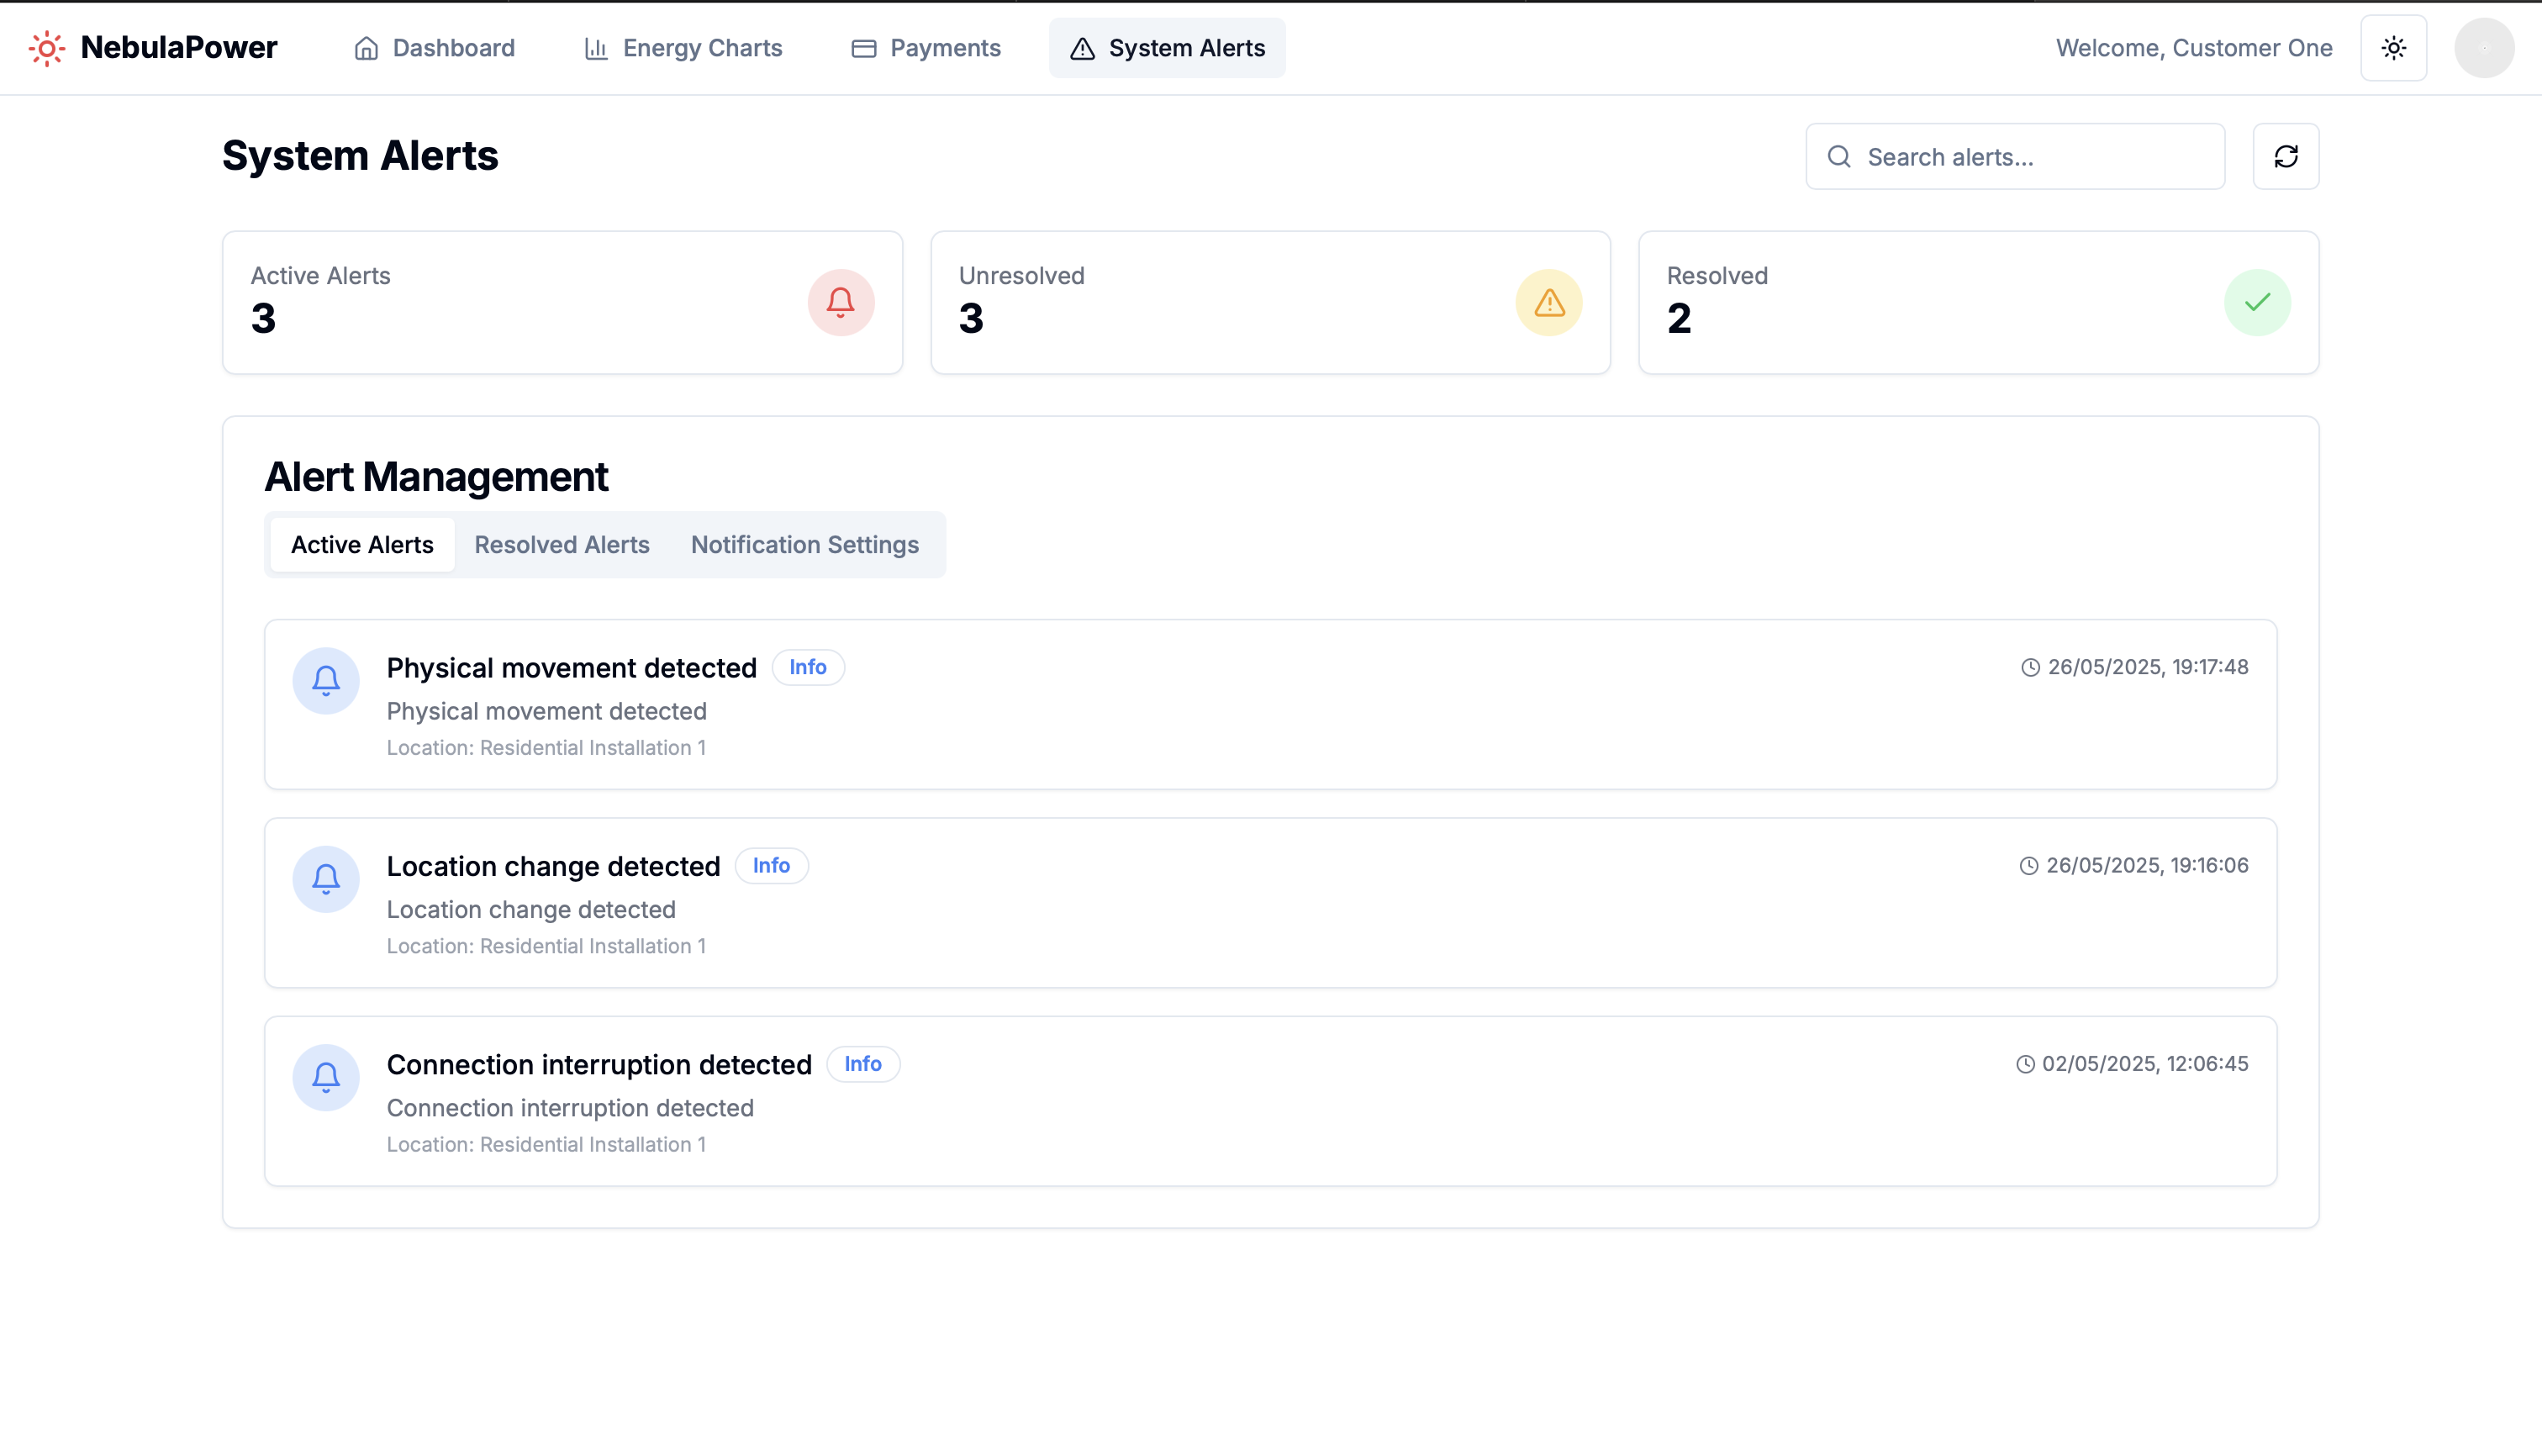
\includegraphics[width=0.85\textwidth]{images_2/customer_alert.png}
    \caption{Customer security alerts}
    \label{fig:security-alerts-customer}
\end{figure}

\subsubsection{System Logs}

\textbf{Operational Logs:} Service logs, errors/warnings, start/stop events, connection status. \textbf{Security Logs:} Audit logs, tamper detection, authentication attempts, authorization violations. Logs support filtering, search, and export (Figures~\ref{fig:system-logs}-\ref{fig:log-status}).

\begin{figure}[h]
    \centering
    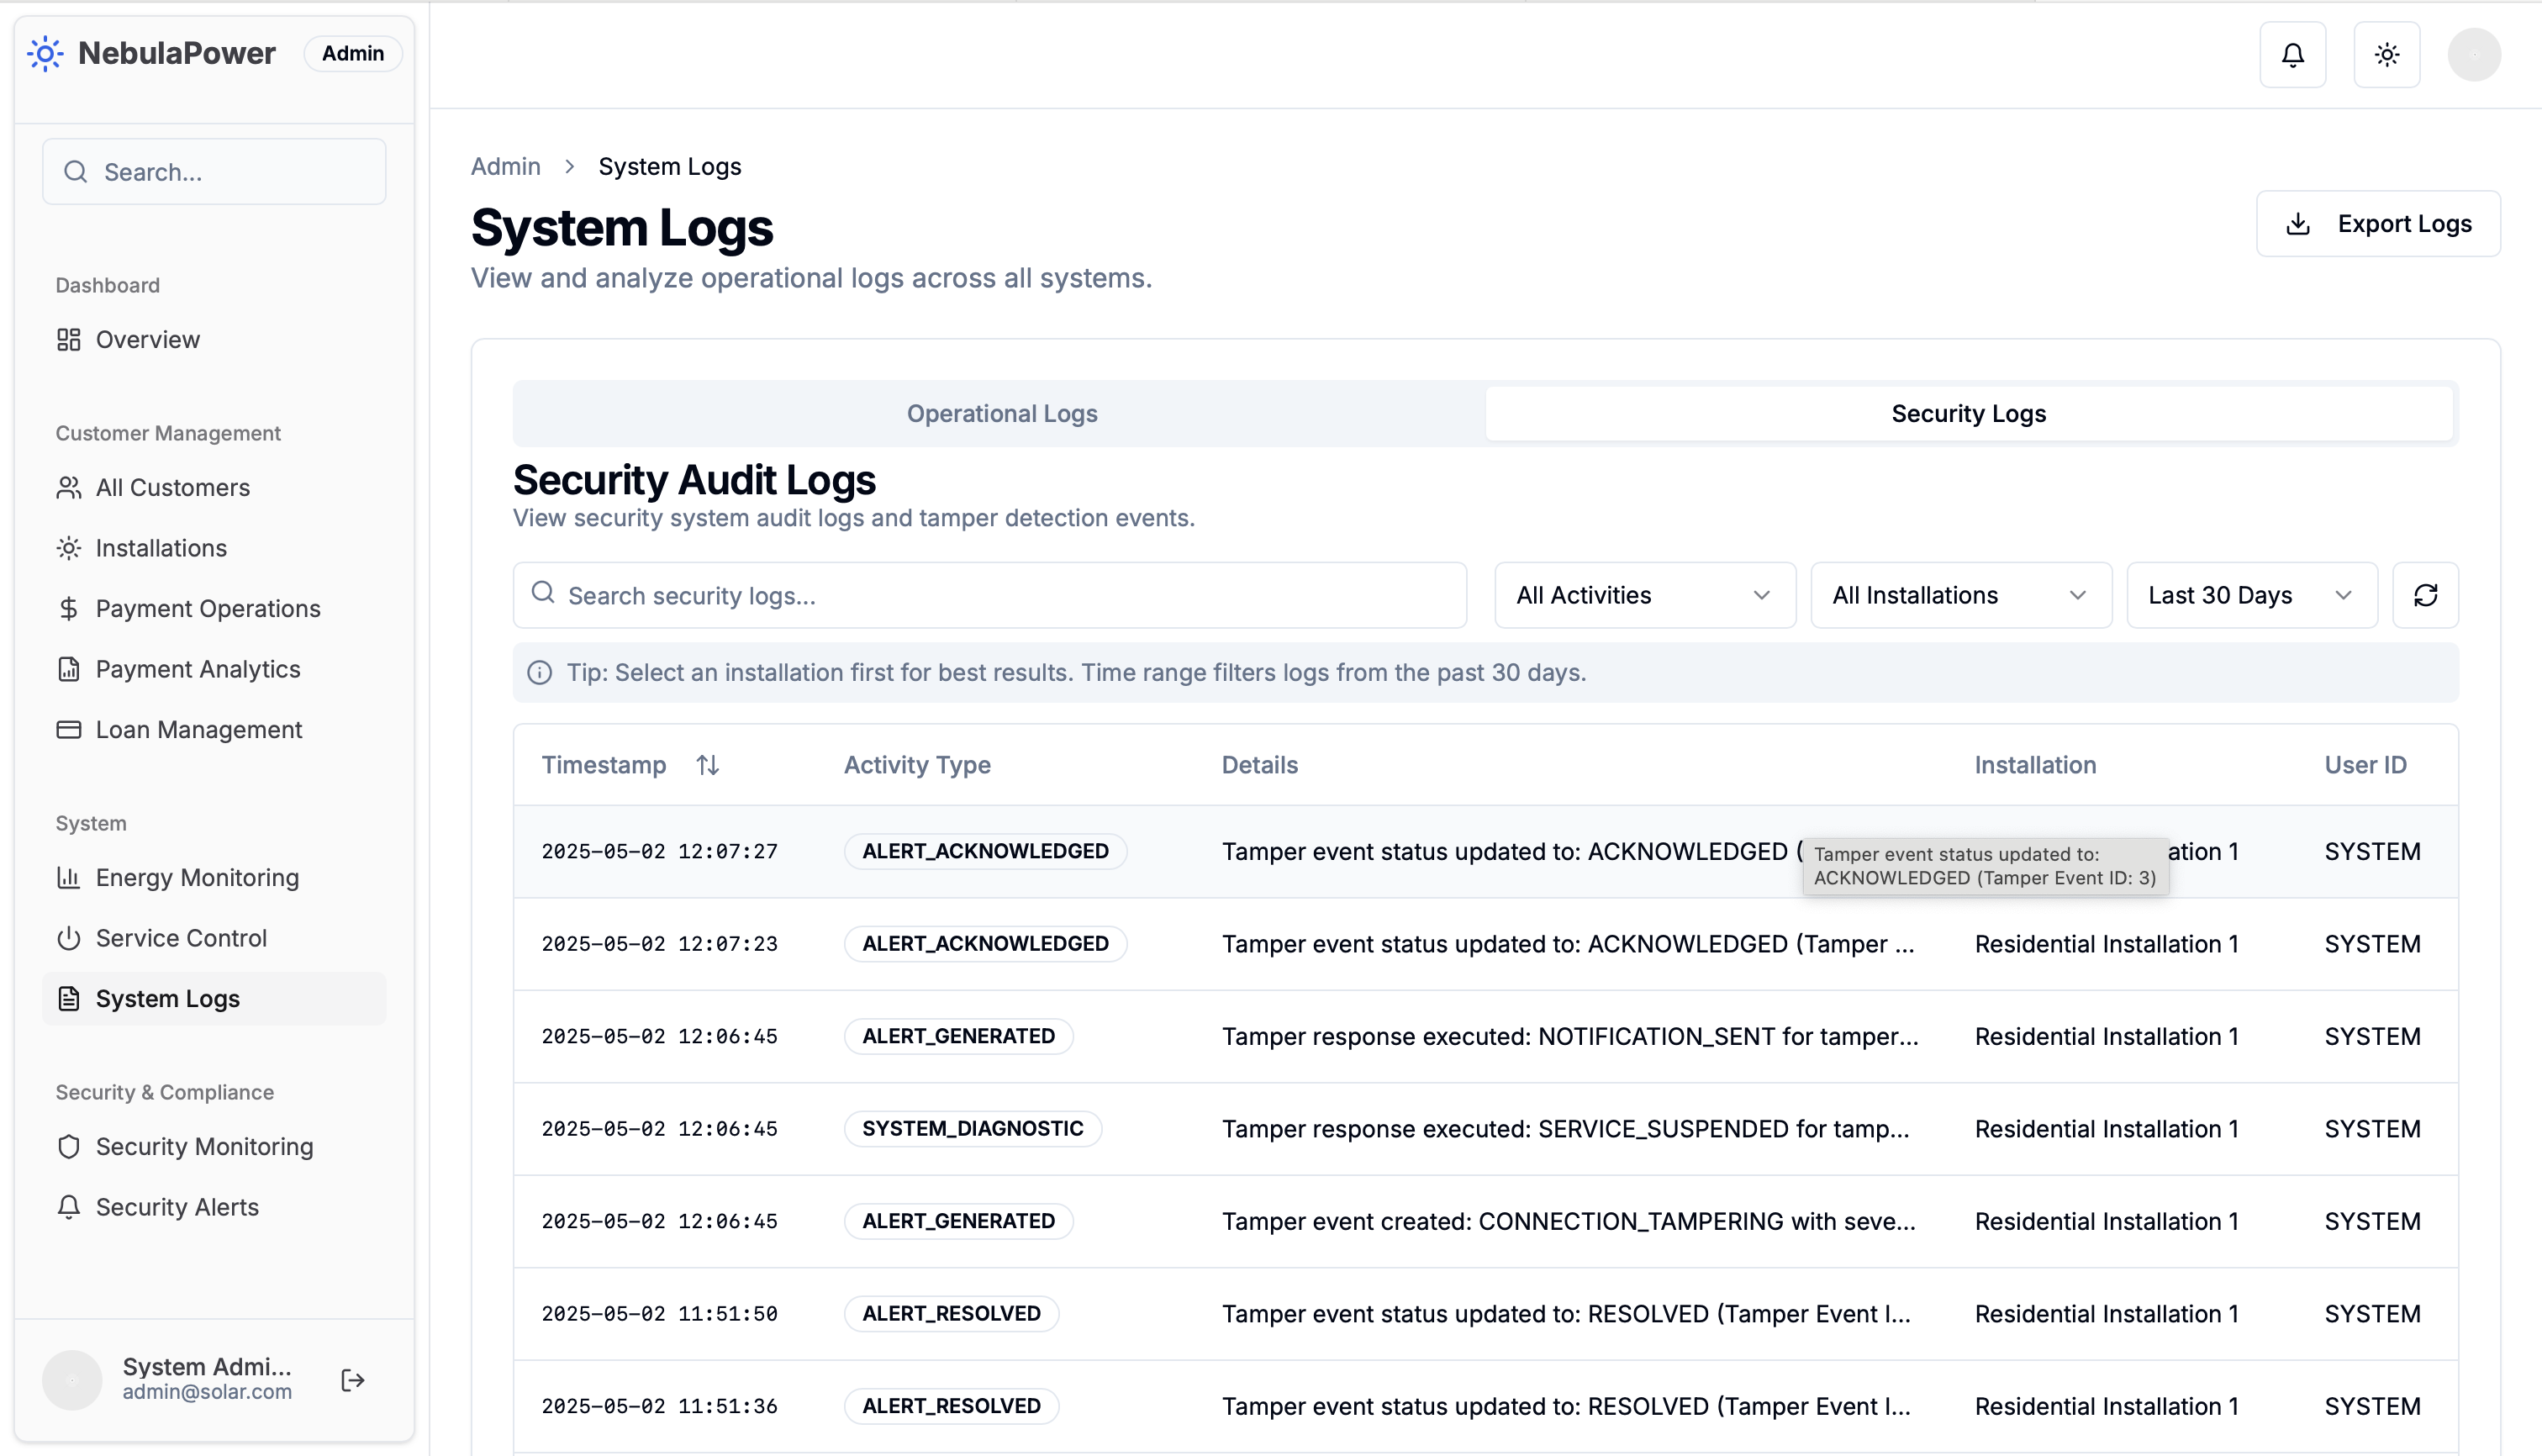
\includegraphics[width=0.8\textwidth]{images_2/admin_system_logs.png}
    \caption{System logs}
    \label{fig:system-logs}
\end{figure}

\begin{figure}[h]
    \centering
    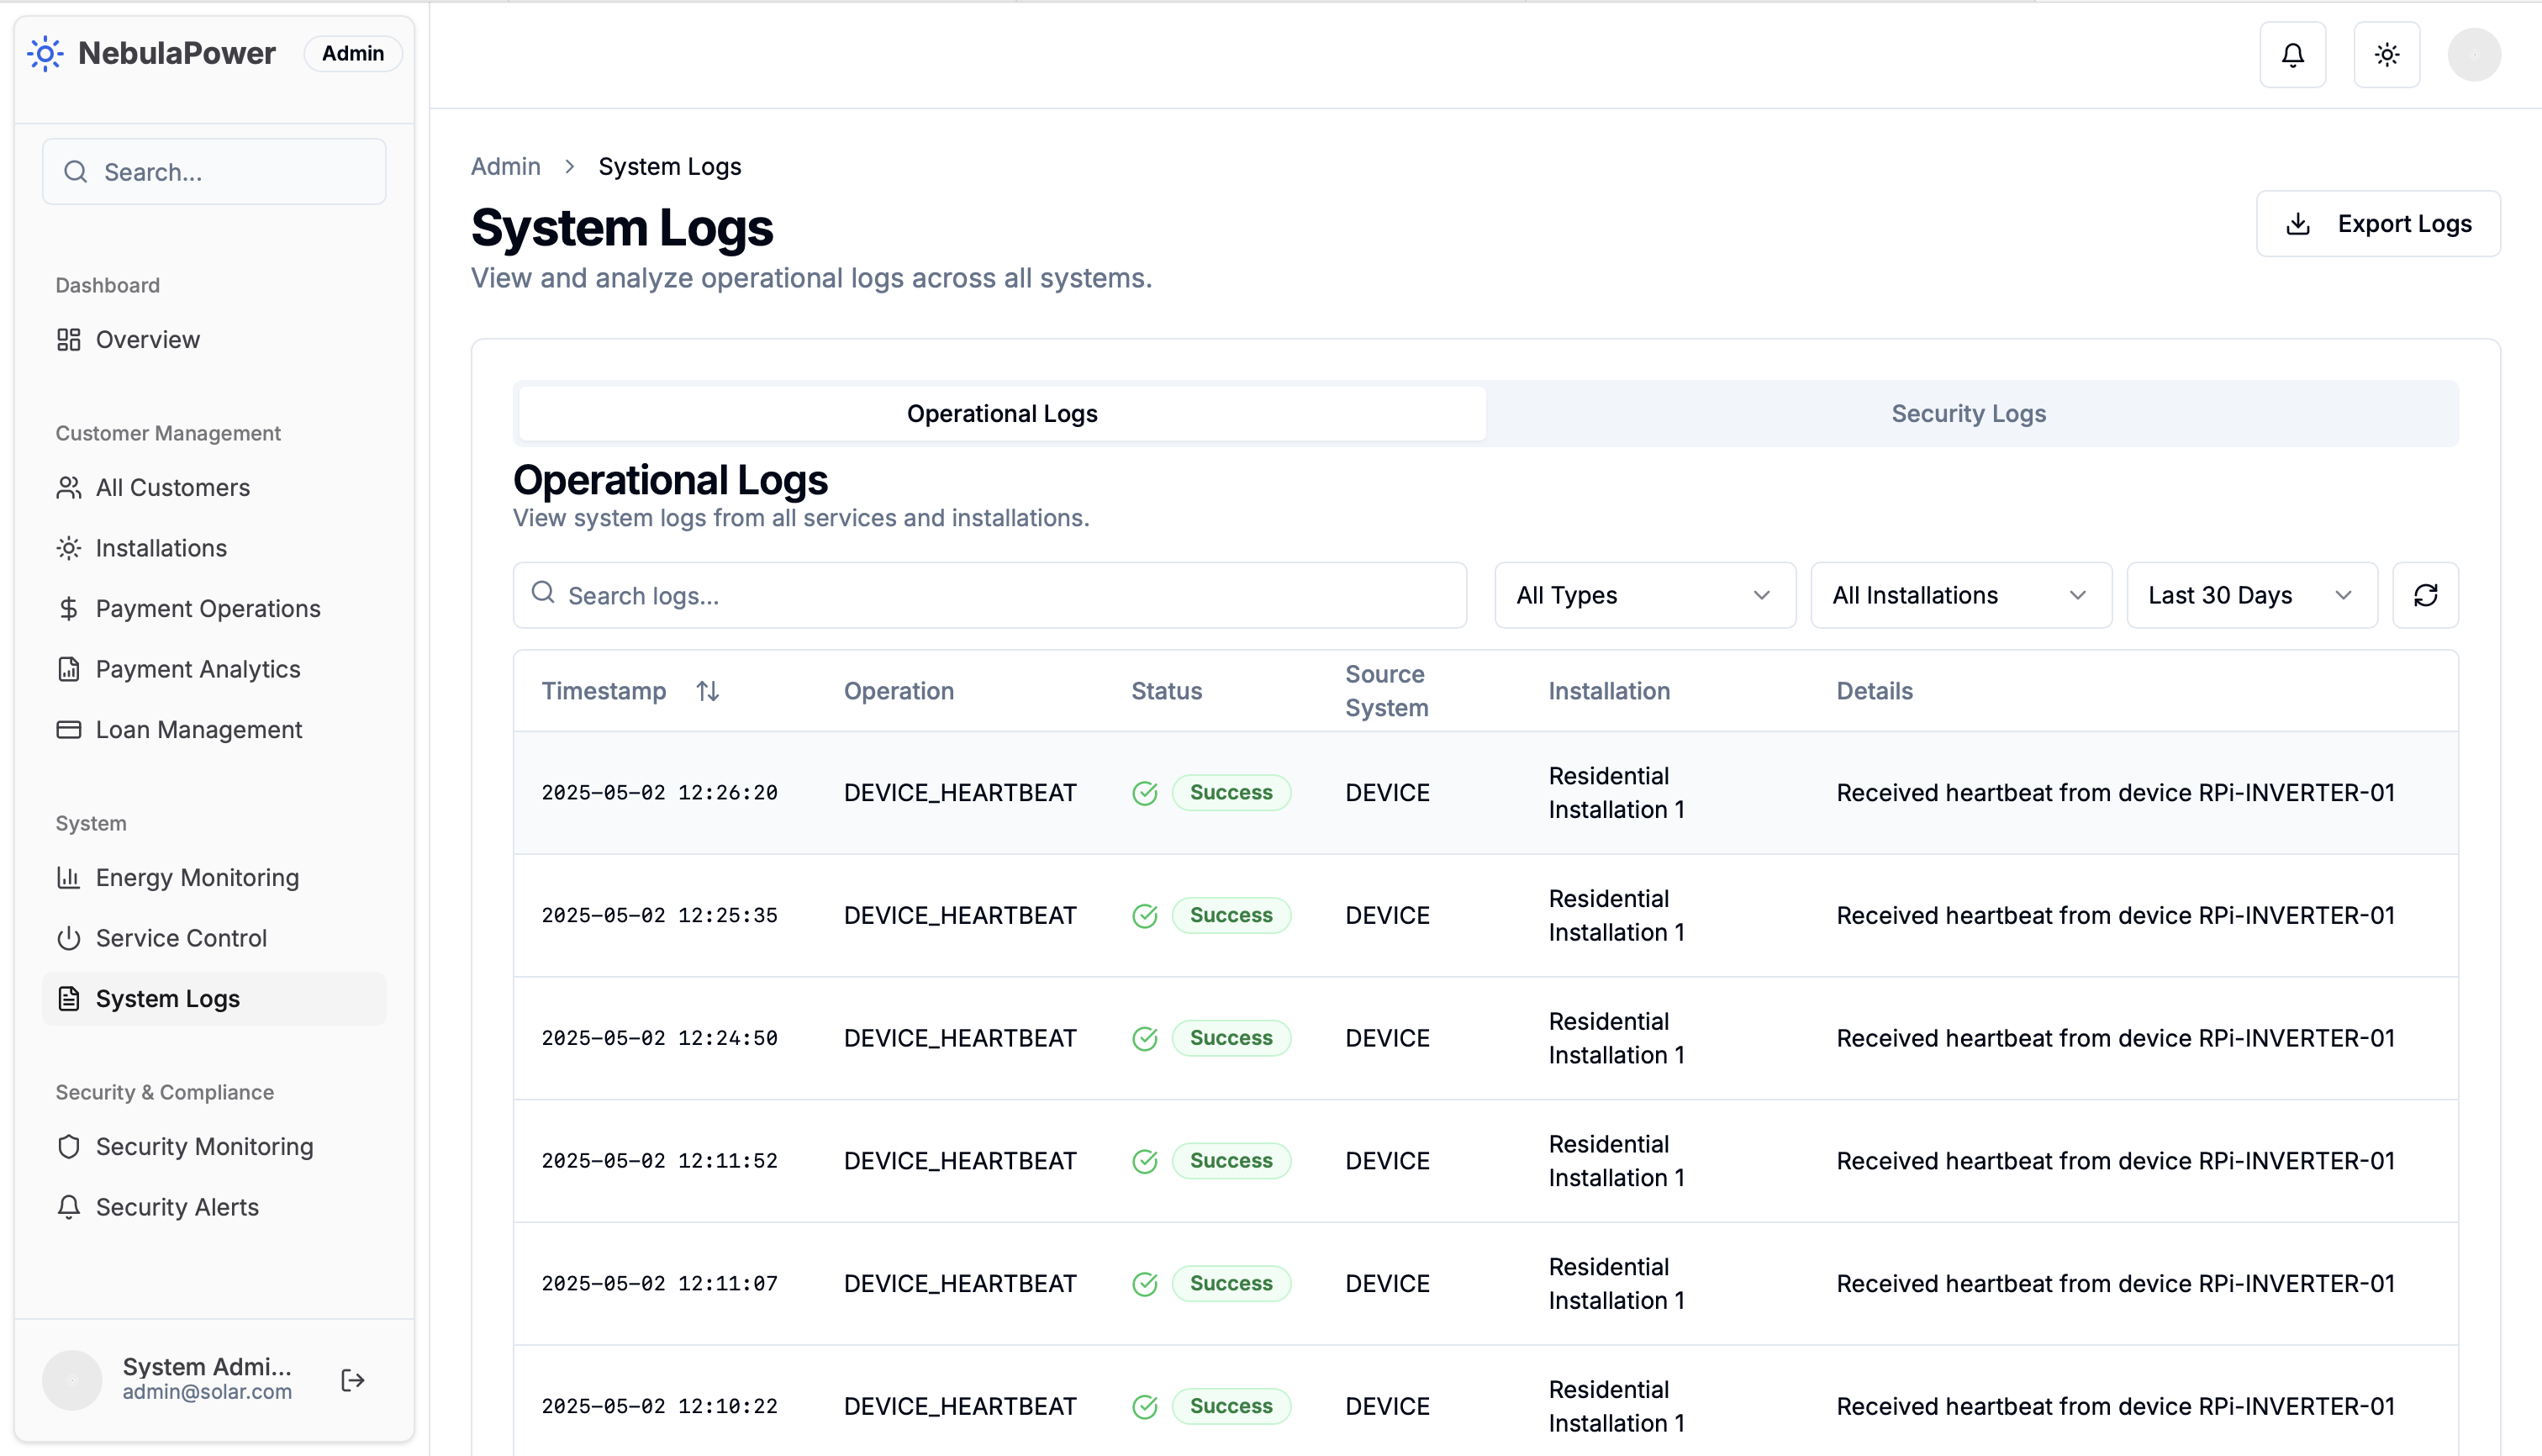
\includegraphics[width=0.8\textwidth]{images_2/admin_op_logs.png}
    \caption{Operational logs}
    \label{fig:operational-logs}
\end{figure}

\begin{figure}[h]
    \centering
    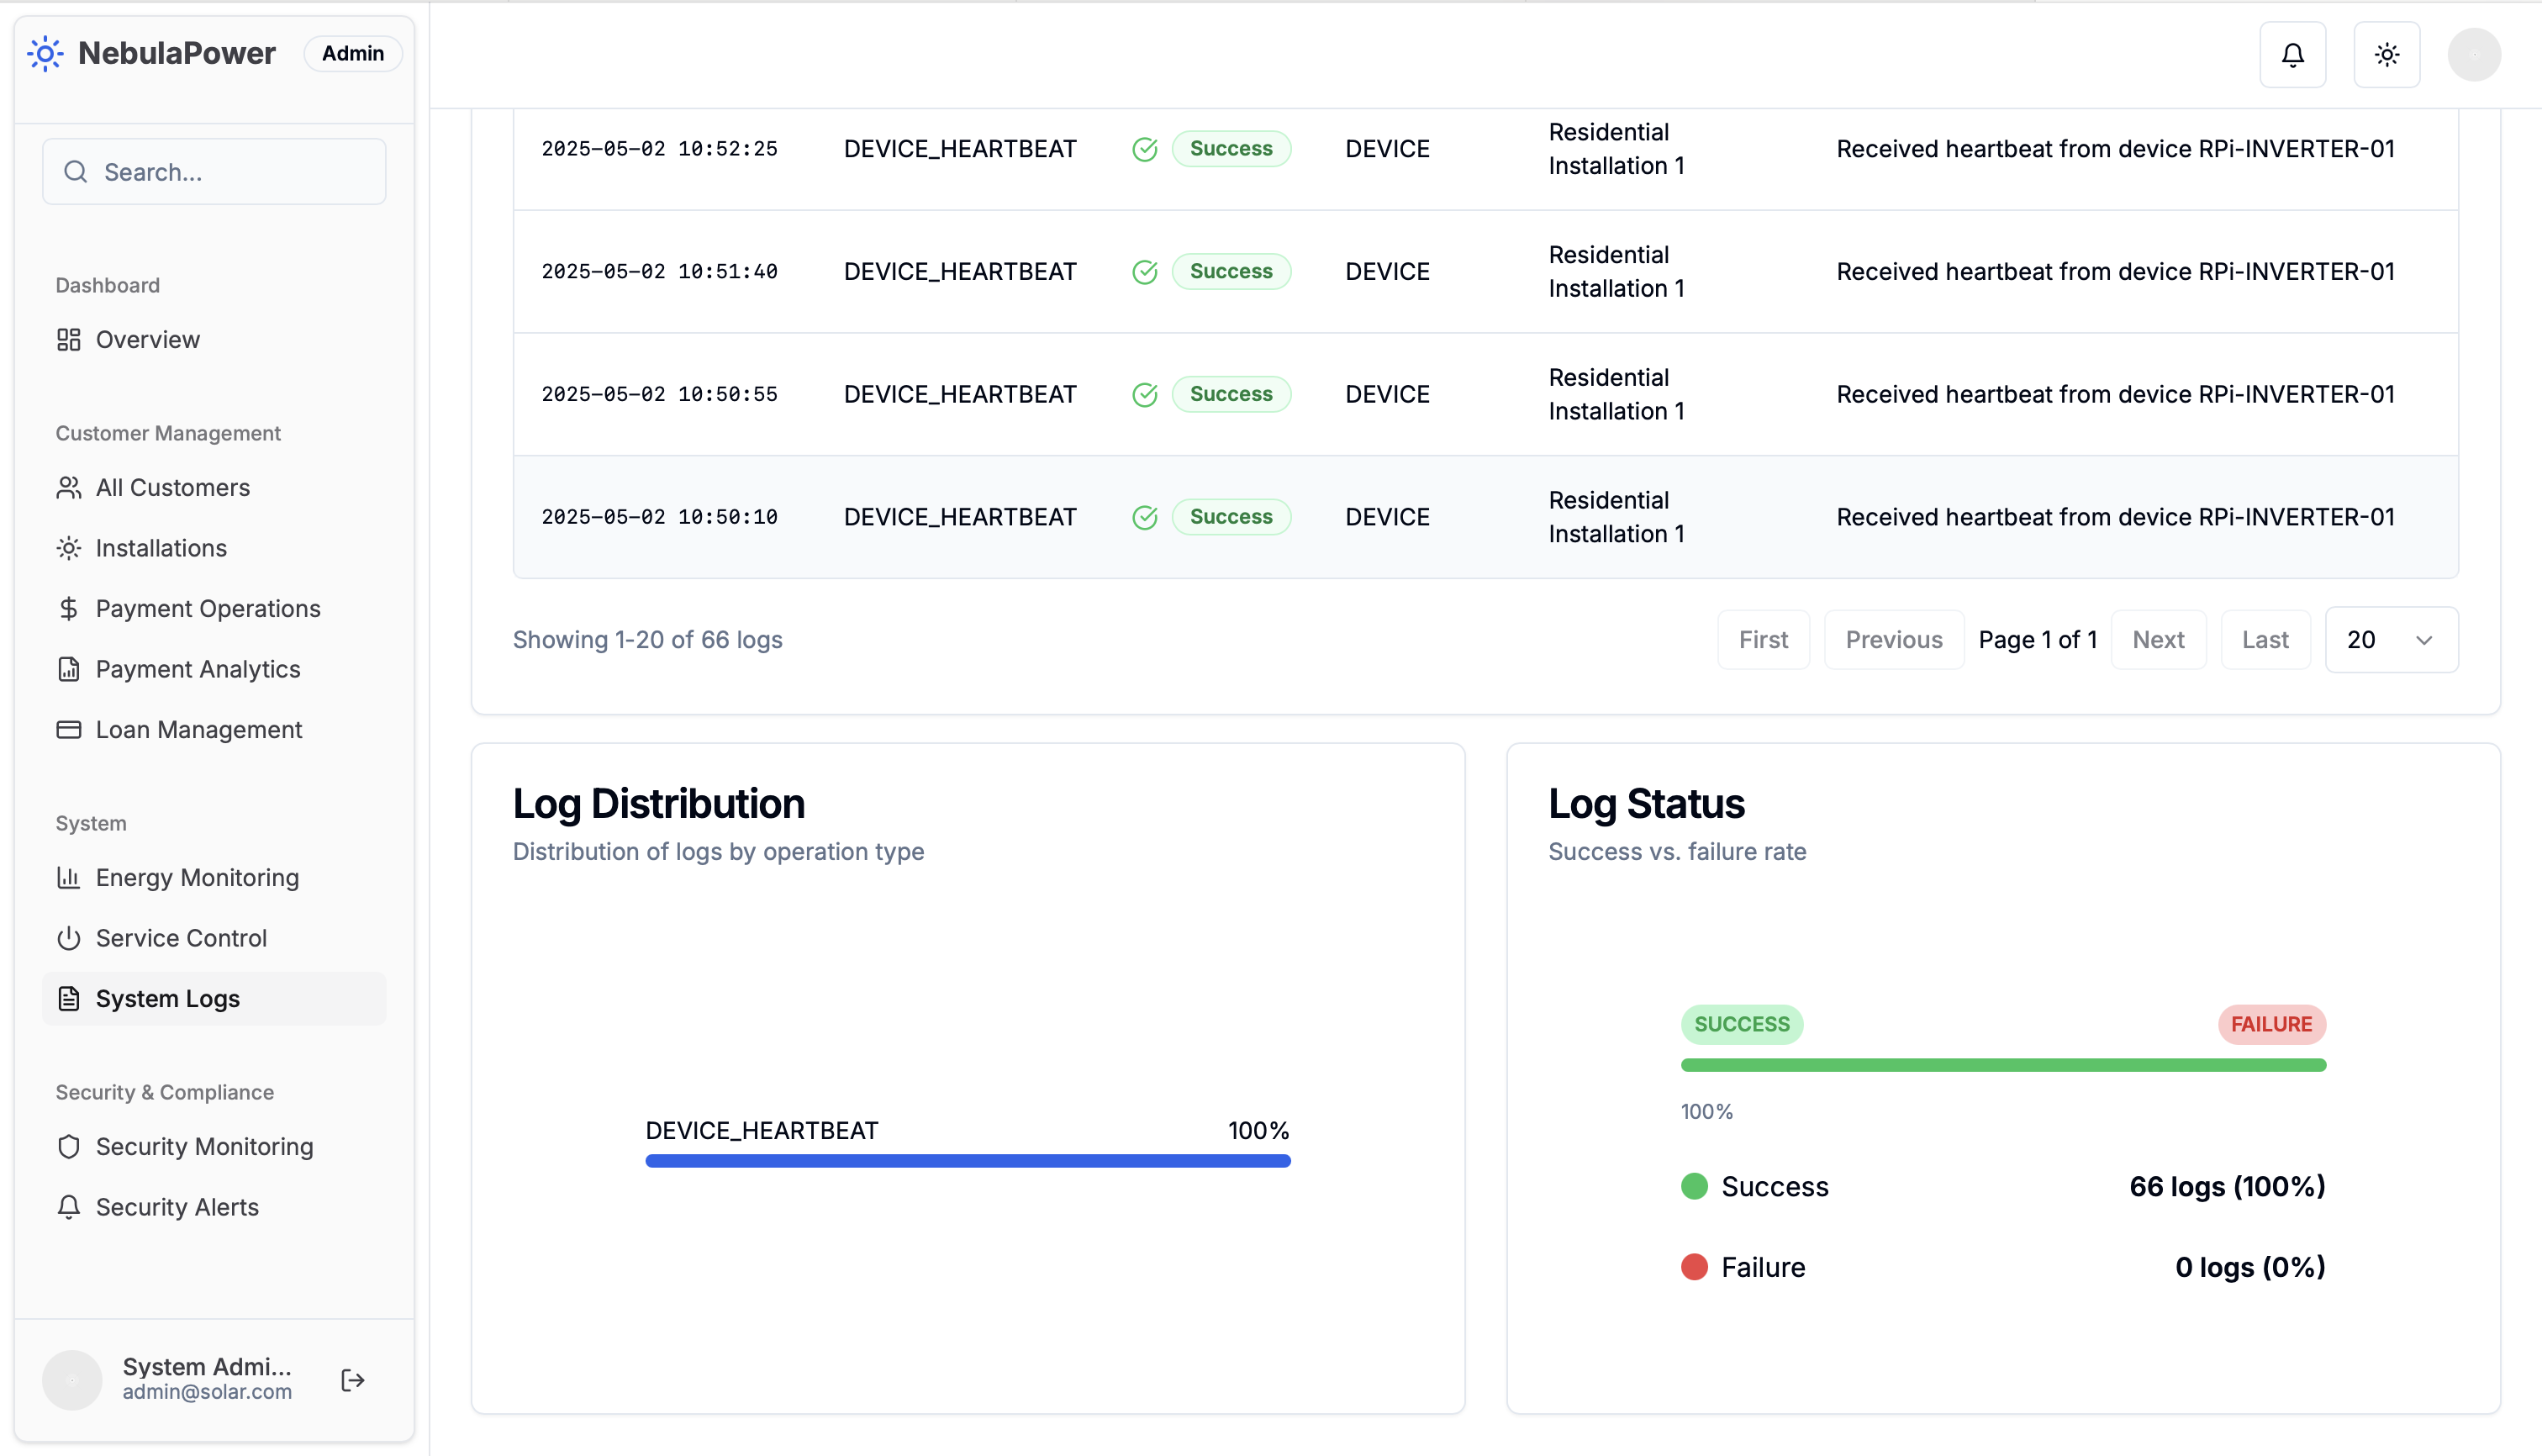
\includegraphics[width=0.8\textwidth]{images_2/admin_op_log_status.png}
    \caption{Log status dashboard}
    \label{fig:log-status}
\end{figure}

\section{Operational Procedures}
\label{sec:operational-procedures}

\textbf{Adding Installation:} Customer Management $\rightarrow$ Installations $\rightarrow$ Add New $\rightarrow$ enter name, capacity, location, customer $\rightarrow$ assign payment plan $\rightarrow$ activate.

\textbf{Deactivating Account:} Customer Management $\rightarrow$ select customer $\rightarrow$ Deactivate Account $\rightarrow$ provide reason $\rightarrow$ confirm.

\textbf{Creating Loan:} Payment Operations $\rightarrow$ Loan Management $\rightarrow$ Add New Loan $\rightarrow$ enter details (name, amount, frequency, duration, rate, customer) $\rightarrow$ Create Payment.

\textbf{Modifying Loan:} Loan Management $\rightarrow$ Edit $\rightarrow$ update parameters $\rightarrow$ save.

\textbf{Manual Payment:} Customer payment history $\rightarrow$ Record Manual Payment $\rightarrow$ enter amount, date, method, reference $\rightarrow$ confirm.

\section{Troubleshooting}
\label{sec:troubleshooting}

\textbf{Authentication Issues:} Verify credentials, check account status, contact administrator if locked.

\textbf{System Access:} Ensure stable internet connection, clear browser cache, try alternate browser.

\textbf{Data Display:} Refresh page, check installation status, verify device simulation is running.

\textbf{Support:} Contact thesis supervisor for research environment issues; provide account email, browser details, error messages.

\section{System Messages and Error Handling}
\label{sec:system-messages}

Common system messages include authentication status ("Login successful", "Invalid credentials"), data operation confirmations ("Created successfully", "Updated successfully"), and error states. For detailed error handling, refer to system logs.
        \begin{itemize}
            \item Installation Name: Descriptive name for the solar installation
            \item Capacity (kW): Total installed solar panel capacity
            \item Location: Physical address of installation
            \item Installation Date: Date when system was installed
        \end{itemize}
        \item Save installation details
    \end{itemize}
    
    \item \textbf{Configure Payment Plan}
    \begin{itemize}
        \item Navigate to Payment Operations $\rightarrow$ Loan Management
        \item Click "Add New Loan"
        \item Configure loan parameters:
        \begin{itemize}
            \item Loan Type: Select from available financing options
            \item Payment Amount: Monthly payment amount
            \item Payment Frequency: Usually monthly
            \item Total Duration: Number of payments or months
            \item Interest Rate: If applicable
        \end{itemize}
        \item Assign loan to the customer
        \item Activate the payment plan
    \end{itemize}
\end{enumerate}

\textbf{Expected Results:}
\begin{itemize}
    \item Customer receives activation email within 5 minutes
    \item Customer account shows "Active" status after email confirmation
    \item Installation appears in Energy Monitoring dashboard
    \item Payment plan is visible in customer's payment tab
    \item System begins collecting simulated data for the installation
\end{itemize}

\subsubsection{Security Alert Response Workflow}
This workflow describes how administrators should respond to security alerts in the system.

\textbf{Workflow Steps:}

\begin{enumerate}
    \item \textbf{Alert Detection and Notification}
    \begin{itemize}
        \item Security alert appears in the administrator dashboard
        \item Alert notification shows in the top navigation bar
        \item System may send email notification (if configured)
    \end{itemize}
    
    \item \textbf{Initial Alert Assessment}
    \begin{itemize}
        \item Navigate to Security \& Compliance $\rightarrow$ Security Alerts
        \item Review alert details:
        \begin{itemize}
            \item Alert severity level (Critical, High, Medium, Low)
            \item Affected installation or system component
            \item Timestamp of detection
            \item Alert description and potential impact
        \end{itemize}
    \end{itemize}
    
    \item \textbf{Alert Investigation}
    \begin{itemize}
        \item Click on alert to view detailed information
        \item Review related system logs in System $\rightarrow$ System Logs
        \item Check installation status in Energy Monitoring
        \item Correlate with any customer-reported issues
    \end{itemize}
    
    \item \textbf{Response Actions}
    \begin{itemize}
        \item For Critical Alerts:
        \begin{itemize}
            \item Immediately contact field technician if available
            \item Notify customer of potential security issue
            \item Document response actions in alert notes
        \end{itemize}
        \item For Lower Priority Alerts:
        \begin{itemize}
            \item Schedule investigation within appropriate timeframe
            \item Assign alert to appropriate team member
            \item Set follow-up reminders
        \end{itemize}
    \end{itemize}
    
    \item \textbf{Resolution and Documentation}
    \begin{itemize}
        \item Update alert status as investigation progresses
        \item Document findings and actions taken
        \item Mark alert as resolved when issue is addressed
        \item Update security procedures if necessary
    \end{itemize}
\end{enumerate}

\subsection{Customer Workflows}
\label{subsec:customer-workflows}

\subsubsection{Daily Energy Monitoring Routine}
This workflow helps customers establish a routine for monitoring their solar installation performance.

\textbf{Workflow Steps:}

\begin{enumerate}
    \item \textbf{Access Customer Dashboard}
    \begin{itemize}
        \item Log in to the Solar Energy Monitoring and Control System platform
        \item Navigate to the Overview tab (default landing page)
    \end{itemize}
    
    \item \textbf{Review Installation Summary}
    \begin{itemize}
        \item Check installation status indicators
        \item Verify all installations show "Online" status
        \item Note any warning or error indicators
    \end{itemize}
    
    \item \textbf{Monitor Energy Production}
    \begin{itemize}
        \item Review current generation (real-time power output)
        \item Check today's production totals
        \item Compare with previous day's performance
        \item Review monthly production trends
    \end{itemize}
    
    \item \textbf{Check System Efficiency}
    \begin{itemize}
        \item Review efficiency percentage
        \item Note any significant deviations from normal performance
        \item Check environmental impact metrics
    \end{itemize}
    
    \item \textbf{Review Alerts and Notifications}
    \begin{itemize}
        \item Check for any security alerts
        \item Review system notifications
        \item Address any required actions
    \end{itemize}
\end{enumerate}

\subsubsection{Payment Review and Management Workflow}
This workflow guides customers through reviewing their payment status and history.

\textbf{Workflow Steps:}

\begin{enumerate}
    \item \textbf{Access Payment Information}
    \begin{itemize}
        \item Navigate to the Payments tab in customer dashboard
        \item Review loan summary information
    \end{itemize}
    
    \item \textbf{Check Payment Progress}
    \begin{itemize}
        \item Review payment progress bar
        \item Note percentage of loan completed
        \item Check remaining payment amount
    \end{itemize}
    
    \item \textbf{Review Payment History}
    \begin{itemize}
        \item Scroll through list of completed payments
        \item Verify payment dates and amounts
        \item Check for any missed or late payments
    \end{itemize}
    
    \item \textbf{Upcoming Payment Planning}
    \begin{itemize}
        \item Review next payment due date
        \item Note payment amount and method
        \item Ensure adequate funds are available
    \end{itemize}
    
    \item \textbf{Address Payment Issues}
    \begin{itemize}
        \item Contact administrator for payment discrepancies
        \item Report any payment processing issues
        \item Request payment plan modifications if needed
    \end{itemize}
\end{enumerate}

\section{System Messages and Error Handling}
\label{sec:system-messages}

This section documents all system messages, notifications, and error conditions that users may encounter while using the Solar Energy Monitoring and Control System. Understanding these messages helps users respond appropriately to different system states.

\subsection{Authentication and Access Messages}
\label{subsec:auth-messages}

\subsubsection{Login and Session Messages}

\textbf{Successful Authentication:}
\begin{itemize}
    \item \texttt{Message}: "Welcome back! Login successful."
    \item \texttt{Context}: Displayed after successful user authentication
    \item \texttt{User Action}: User is redirected to appropriate dashboard
\end{itemize}

\textbf{Invalid Credentials:}
\begin{itemize}
    \item \texttt{Message}: "Invalid email or password. Please check your credentials and try again."
    \item \texttt{Context}: Displayed when login attempt fails due to incorrect credentials
    \item \texttt{User Action}: Re-enter correct username and password
\end{itemize}

\textbf{Account Locked:}
\begin{itemize}
    \item \texttt{Message}: "Account temporarily locked due to multiple failed login attempts. Please try again in 15 minutes or contact support."
    \item \texttt{Context}: Displayed after exceeding failed login attempt threshold
    \item \texttt{User Action}: Wait for lockout period to expire or contact administrator
\end{itemize}

\textbf{Session Expired:}
\begin{itemize}
    \item \texttt{Message}: "Your session has expired for security reasons. Please log in again."
    \item \texttt{Context}: Displayed when user session timeout is reached
    \item \texttt{User Action}: Re-authenticate to continue using the system
\end{itemize}

\textbf{Insufficient Privileges:}
\begin{itemize}
    \item \texttt{Message}: "You do not have permission to access this feature. Contact your administrator if you believe this is an error."
    \item \texttt{Context}: Displayed when user attempts to access restricted functionality
    \item \texttt{User Action}: Contact administrator to request appropriate permissions
\end{itemize}

\subsection{Data Operation Messages}
\label{subsec:data-messages}

\subsubsection{Create Operations}

\textbf{Successful Creation:}
\begin{itemize}
    \item \texttt{Message}: "[Item] created successfully."
    \item \texttt{Context}: Displayed after successful creation of customers, installations, loans, etc.
    \item \texttt{User Action}: Continue with workflow or navigate to view created item
\end{itemize}

\textbf{Validation Errors:}
\begin{itemize}
    \item \texttt{Message}: "Please correct the following errors: [detailed field-specific error list]"
    \item \texttt{Context}: Displayed when form submission contains invalid data
    \item \texttt{User Action}: Correct highlighted fields and resubmit form
\end{itemize}

\textbf{Duplicate Data:}
\begin{itemize}
    \item \texttt{Message}: "A [record type] with this [field] already exists. Please use a different value."
    \item \texttt{Context}: Displayed when attempting to create record with non-unique required fields
    \item \texttt{User Action}: Modify field value to be unique and resubmit
\end{itemize}

\subsubsection{Update Operations}

\textbf{Successful Update:}
\begin{itemize}
    \item \texttt{Message}: "[Item] updated successfully."
    \item \texttt{Context}: Displayed after successful modification of existing records
    \item \texttt{User Action}: Changes are saved and user can continue with other tasks
\end{itemize}

\textbf{Concurrent Modification:}
\begin{itemize}
    \item \texttt{Message}: "This record has been modified by another user. Please refresh and try again."
    \item \texttt{Context}: Displayed when attempting to save changes to a record that was modified by another user
    \item \texttt{User Action}: Refresh page and re-apply changes
\end{itemize}

\subsubsection{Delete Operations}

\textbf{Confirmation Required:}
\begin{itemize}
    \item \texttt{Message}: "Are you sure you want to delete [item]? This action cannot be undone."
    \item \texttt{Context}: Displayed as confirmation dialog before deletion
    \item \texttt{User Action}: Confirm deletion or cancel operation
\end{itemize}

\textbf{Successful Deletion:}
\begin{itemize}
    \item \texttt{Message}: "[Item] deleted successfully."
    \item \texttt{Context}: Displayed after successful deletion
    \item \texttt{User Action}: Item is removed from lists and user is returned to parent view
\end{itemize}

\textbf{Deletion Restricted:}
\begin{itemize}
    \item \texttt{Message}: "Cannot delete [item] because it is referenced by other records. Please remove dependencies first."
    \item \texttt{Context}: Displayed when attempting to delete records with dependencies
    \item \texttt{User Action}: Remove or reassign dependent records before attempting deletion
\end{itemize}

\subsection{System Status and Monitoring Messages}
\label{subsec:system-status-messages}

\subsubsection{Installation Status Messages}

\textbf{Online Status:}
\begin{itemize}
    \item \texttt{Message}: "Installation [name] is online and functioning normally."
    \item \texttt{Context}: Displayed when installation is communicating and producing expected data
    \item \texttt{User Action}: No action required; normal monitoring continues
\end{itemize}

\textbf{Offline Status:}
\begin{itemize}
    \item \texttt{Message}: "Installation [name] is offline. Last communication: [timestamp]."
    \item \texttt{Context}: Displayed when installation has not communicated within expected timeframe
    \item \texttt{User Action}: Customer should contact administrator; administrator should investigate connectivity
\end{itemize}

\textbf{Performance Warning:}
\begin{itemize}
    \item \texttt{Message}: "Installation [name] is performing below expected efficiency. Current: [value]\%, Expected: [value]\%."
    \item \texttt{Context}: Displayed when installation efficiency drops below threshold
    \item \texttt{User Action}: Monitor for improvement; contact support if condition persists
\end{itemize}

\subsubsection{Security Alert Messages}

\textbf{Tampering Detection:}
\begin{itemize}
    \item \texttt{Message}: "Security Alert: Potential tampering detected at installation [name]. Immediate attention required."
    \item \texttt{Context}: Displayed when security monitoring detects potential unauthorized access
    \item \texttt{User Action}: Administrator should investigate immediately; customer should verify installation security
\end{itemize}

\textbf{Unusual Activity:}
\begin{itemize}
    \item \texttt{Message}: "Security Notice: Unusual activity patterns detected at installation [name]. Monitoring enhanced."
    \item \texttt{Context}: Displayed when system detects patterns that may indicate security concerns
    \item \texttt{User Action}: Monitor situation; investigate if patterns continue
\end{itemize}

\subsection{Technical Error Messages}
\label{subsec:technical-errors}

\subsubsection{Connectivity Issues}

\textbf{Database Connection Error:}
\begin{itemize}
    \item \texttt{Message}: "Temporary system unavailability. Please try again in a few minutes."
    \item \texttt{Context}: Displayed when database connectivity issues occur
    \item \texttt{User Action}: Wait and retry operation; contact support if problem persists
\end{itemize}

\textbf{Network Timeout:}
\begin{itemize}
    \item \texttt{Message}: "Request timed out. Please check your internet connection and try again."
    \item \texttt{Context}: Displayed when network request exceeds timeout threshold
    \item \texttt{User Action}: Verify internet connectivity and retry operation
\end{itemize}

\subsubsection{Application Errors}

\textbf{Unexpected Error:}
\begin{itemize}
    \item \texttt{Message}: "An unexpected error occurred. Please refresh the page and try again. If the problem persists, contact support with error code: [code]."
    \item \texttt{Context}: Displayed when unhandled exceptions occur
    \item \texttt{User Action}: Refresh page and retry; contact support with error code if problem continues
\end{itemize}

\textbf{Feature Unavailable:}
\begin{itemize}
    \item \texttt{Message}: "This feature is temporarily unavailable for maintenance. Please try again later."
    \item \texttt{Context}: Displayed when specific system features are disabled for maintenance
    \item \texttt{User Action}: Wait for maintenance completion and retry
\end{itemize}

\section{Security and Troubleshooting Instructions}
\label{sec:security-troubleshooting}

This section provides comprehensive guidance on security best practices, common issues, and troubleshooting procedures for the Solar Energy Monitoring and Control System.

\subsection{Security Best Practices}
\label{subsec:security-practices}

\subsubsection{Password Security}

\textbf{Password Requirements:}
\begin{itemize}
    \item Minimum 8 characters in length
    \item Must contain at least one uppercase letter (A-Z)
    \item Must contain at least one lowercase letter (a-z)
    \item Must contain at least one number (0-9)
    \item Must contain at least one special character (!@\#\$\%\textasciicircum\&*)
    \item Cannot be the same as the previous 5 passwords
    \item Cannot contain common dictionary words or personal information
\end{itemize}

\textbf{Password Management Guidelines:}
\begin{itemize}
    \item Change passwords every 90 days (configurable by administrator)
    \item Never share passwords with other users
    \item Use different passwords for different systems
    \item Consider using a reputable password manager
    \item Report suspected password compromise immediately
\end{itemize}

\subsubsection{Session Security}

\textbf{Session Management:}
\begin{itemize}
    \item Always log out when finished using the system
    \item Do not leave unattended sessions open
    \item Sessions automatically expire after 30 minutes of inactivity
    \item Avoid using shared or public computers for sensitive operations
    \item Clear browser cache and cookies after use on shared computers
\end{itemize}

\textbf{Browser Security:}
\begin{itemize}
    \item Ensure browser is updated to the latest version
    \item Enable automatic security updates
    \item Disable password saving for the NebulaPower platform
    \item Use private/incognito browsing mode on shared computers
    \item Verify HTTPS connection (look for lock icon in address bar)
\end{itemize}

\subsubsection{Data Protection}

\textbf{Information Handling:}
\begin{itemize}
    \item Do not share login credentials with unauthorized persons
    \item Report any suspected security incidents immediately
    \item Verify recipient before sharing sensitive installation data
    \item Use secure communication channels for sensitive discussions
    \item Regularly review account activity for unusual patterns
\end{itemize}

\subsection{Common Issues and Solutions}
\label{subsec:common-issues}

\subsubsection{Login and Authentication Issues}

\textbf{Problem}: Cannot remember password
\begin{itemize}
    \item \textbf{Solution}: Use "Forgot Password" link on login page
    \item \textbf{Steps}:
    \begin{enumerate}
        \item Click "Forgot Password" on login page
        \item Enter registered email address
        \item Check email for password reset link
        \item Follow link and create new password
        \item Login with new password
    \end{enumerate}
    \item \textbf{Contact Support}: If no email is received within 10 minutes
\end{itemize}

\textbf{Problem}: Account appears to be locked
\begin{itemize}
    \item \textbf{Cause}: Too many failed login attempts
    \item \textbf{Solution}: Wait 15 minutes for automatic unlock
    \item \textbf{Prevention}: Ensure caps lock is off; type password carefully
    \item \textbf{Contact Support}: If lockouts occur frequently
\end{itemize}

\textbf{Problem}: Session keeps expiring quickly
\begin{itemize}
    \item \textbf{Cause}: Browser not accepting cookies or system security settings
    \item \textbf{Solution}:
    \begin{enumerate}
        \item Enable cookies in browser settings
        \item Add platform to browser's trusted sites
        \item Clear browser cache and cookies
        \item Restart browser and try again
    \end{enumerate}
\end{itemize}

\subsubsection{Dashboard and Interface Issues}

\textbf{Problem}: Dashboard not loading completely
\begin{itemize}
    \item \textbf{Cause}: JavaScript disabled, slow connection, or browser compatibility
    \item \textbf{Solution}:
    \begin{enumerate}
        \item Verify JavaScript is enabled in browser
        \item Check internet connection speed
        \item Try refreshing the page (F5 or Ctrl+F5)
        \item Clear browser cache and cookies
        \item Try different browser if problem persists
    \end{enumerate}
\end{itemize}

\textbf{Problem}: Charts and graphs not displaying
\begin{itemize}
    \item \textbf{Cause}: Browser compatibility, plugins, or data loading issues
    \item \textbf{Solution}:
    \begin{enumerate}
        \item Ensure browser meets minimum requirements
        \item Disable browser extensions temporarily
        \item Check for browser updates
        \item Allow pop-ups from the platform domain
    \end{enumerate}
\end{itemize}

\textbf{Problem}: Interface appears broken or misaligned
\begin{itemize}
    \item \textbf{Cause}: Browser compatibility or cached resources
    \item \textbf{Solution}:
    \begin{enumerate}
        \item Clear browser cache and reload page
        \item Try different browser
        \item Check screen resolution meets minimum requirements
        \item Ensure browser zoom is set to 100\%
    \end{enumerate}
\end{itemize}

\subsubsection{Data and Monitoring Issues}

\textbf{Problem}: Installation showing as offline
\begin{itemize}
    \item \textbf{For Customers}:
    \begin{enumerate}
        \item Wait 5-10 minutes and refresh dashboard
        \item Check if other installations are also offline
        \item Contact administrator if issue persists
    \end{enumerate}
    \item \textbf{For Administrators}:
    \begin{enumerate}
        \item Check system logs for connectivity errors
        \item Verify simulation scripts are running (in research environment)
        \item Check network connectivity to installation hardware
        \item Restart communication services if necessary
    \end{enumerate}
\end{itemize}

\textbf{Problem}: Energy data appears incorrect or missing
\begin{itemize}
    \item \textbf{Verification Steps}:
    \begin{enumerate}
        \item Compare with previous day's data for consistency
        \item Check installation status indicators
        \item Verify time zone settings are correct
        \item Look for any system alerts related to the installation
    \end{enumerate}
    \item \textbf{Contact Support}: If data anomalies persist beyond 24 hours
\end{itemize}

\subsection{Emergency Procedures}
\label{subsec:emergency-procedures}

\subsubsection{Security Incident Response}

\textbf{Suspected Account Compromise:}
\begin{enumerate}
    \item Immediately change password if still possible
    \item Log out of all sessions
    \item Contact administrator immediately
    \item Document any suspicious activity noticed
    \item Monitor account for unauthorized changes
\end{enumerate}

\textbf{Suspected Tampering Alert:}
\begin{enumerate}
    \item Do not ignore security alerts
    \item Contact administrator immediately
    \item Document any unusual observations about the installation
    \item Avoid accessing the installation until cleared by administrator
    \item Cooperate with any security investigation
\end{enumerate}

\subsubsection{System Unavailability}

\textbf{Complete System Outage:}
\begin{itemize}
    \item Check internet connectivity first
    \item Try accessing from different device or network
    \item Wait 15-30 minutes before reporting (may be scheduled maintenance)
    \item Contact administrator if outage extends beyond expected timeframe
    \item Monitor official communication channels for updates
\end{itemize}

\subsection{Contact and Support Information}
\label{subsec:support-info}

\textbf{Technical Support:}
\begin{itemize}
    \item \textbf{For Research Environment}: Contact thesis supervisor or designated technical contact
    \item \textbf{Response Time}: Within 24-48 hours for non-critical issues
    \item \textbf{Emergency Issues}: Use emergency contact procedures defined by organization
\end{itemize}

\textbf{Information to Provide When Reporting Issues:}
\begin{itemize}
    \item User account (email address)
    \item Browser type and version
    \item Operating system
    \item Exact error message (screenshot preferred)
    \item Steps taken before problem occurred
    \item Whether problem affects multiple users or installations
\end{itemize}

This section outlines potential issues that might be encountered during testing and evaluation of the Solar Energy Monitoring and Control System. It is important to note that these troubleshooting guidelines are specific to the thesis research environment and are not intended for production use.

\subsection{Testing Environment Issues}
\label{subsec:testing-troubleshooting}

When testing the system in the research environment, the following issues may occur:

\begin{itemize}
    \item \textbf{Authentication Issues}: During testing, authentication may occasionally fail due to the test environment configuration. This is expected behavior in the current research implementation.
    
    \item \textbf{Data Simulation Limitations}: The simulated data generation may not perfectly replicate real-world scenarios, as it is designed primarily for demonstrating the system's capabilities rather than operational accuracy.
    
    \item \textbf{Interface Responsiveness}: The current interface implementation prioritizes functionality demonstration over performance optimization, which may result in occasional delays when navigating between views.
\end{itemize}

\subsection{Research Implementation Limitations}
\label{subsec:research-limitations}

The current implementation has the following known limitations:

\begin{itemize}
    \item \textbf{Email Integration Not Implemented}: The system does not include email server integration. All email-related functionality (account activation, password reset notifications, payment reminders, security alerts) is simulated for demonstration purposes only. Users cannot receive actual emails from the system.
    
    \item \textbf{Simulated Payment Processing}: Payment functions are simulated for demonstration purposes only and do not connect to actual payment processing systems.
    
    \item \textbf{Limited Data Persistence}: Data persistence across sessions is limited in scope, as the focus is on demonstrating functionality rather than long-term data storage.
    
    \item \textbf{Security Implementation}: Security features are implemented at a conceptual level to demonstrate the architecture's security capabilities, but are not hardened for real-world deployment.
    
    \item \textbf{Simulated Alerts}: Security and system alerts are generated through simulation scripts rather than from actual system events.
\end{itemize}

\subsection{Development Testing Guidance}
\label{subsec:development-testing}

For researchers and developers testing the system:

\begin{itemize}
    \item The system is most stable when tested with the specific browser versions and environments listed in the system requirements section.
    
    \item Simulation scripts may need to be restarted if data streams appear to stop, as this is expected behavior in the research environment.
    
    \item When evaluating functionality, focus on the conceptual demonstration rather than production-ready performance metrics.
\end{itemize}

\section{Reference}
\label{sec:reference}

This section provides reference information for users of the Solar Energy Monitoring and Control System.

\subsection{Glossary}
\label{subsec:glossary}

\begin{description}
    \item[API] Application Programming Interface - A set of rules and protocols for building and interacting with software applications.
    \item[Authentication] The process of verifying the identity of a user or device.
    \item[Authorization] The process of determining what permissions a user has once authenticated.
    \item[Dashboard] A visual interface showing key metrics and status information.
    \item[Device Token] A unique identifier used to authenticate a device with the system.
    \item[Inverter] A device that converts DC electricity from solar panels into AC electricity for home use or grid export.
    \item[kWh (Kilowatt-hour)] A unit of energy equal to 1,000 watt-hours, used to measure electricity consumption and production.
    \item[MFA (Multi-Factor Authentication)] An authentication method requiring users to provide two or more verification factors.
    \item[PAYG (Pay-As-You-Go)] A financing model where customers pay for solar systems in installments as they use them.
    \item[PV (Photovoltaic)] Technology that converts sunlight directly into electricity using semiconductor materials.
    \item[Tampering] Unauthorized modification or interference with a solar installation or monitoring equipment.
    \item[Yield] The amount of electrical energy produced by a solar installation over a specific period.
\end{description}

\textit{Note: Keyboard shortcuts and error code reference features are planned for future versions of the platform.}

\subsection{Research and Development Resources}
\label{subsec:research-resources}

For research, thesis evaluation, and further development of the research concepts:

\begin{itemize}
    \item \textbf{Source Code Documentation}: Comprehensive inline comments and documentation are provided within the codebase to explain implementation details and design decisions.
    
    \item \textbf{Research Framework}: The system serves as a research framework for exploring concepts in renewable energy monitoring, payment compliance, and security monitoring in developing markets.
    
    \item \textbf{Future Research Directions}: Potential areas for extending this research are outlined in the conclusion chapter of this thesis.
\end{itemize}

Complete research documentation, including architectural diagrams and technical specifications, is available in the project repository at \url{https://github.com/2001J/nebular-power/tree/main/docs}.

This system was developed as part of a thesis project exploring solar energy monitoring and financing solutions in developing markets, serving as a research instrument rather than a production-ready solution. It demonstrates the theoretical framework presented in this thesis and provides a platform for empirical validation of the research hypotheses.

\section{Documentation Summary and Compliance}
\label{sec:documentation-summary}

\subsection{Coverage Verification}
This user documentation has been designed to meet comprehensive evaluation criteria for user documentation standards. The following areas have been addressed:

\subsubsection{Target Audience and Task Description}
\begin{itemize}
    \item \textbf{$\checkmark$ Task Description}: Section \ref{sec:system-overview} provides clear description of the Solar Energy Monitoring and Control System's purpose and capabilities
    \item \textbf{$\checkmark$ Target Audience}: Detailed user group specifications with prerequisites and technical requirements for each user type
    \item \textbf{$\checkmark$ User Roles}: Comprehensive role definitions with specific access privileges and responsibilities
\end{itemize}

\subsubsection{System Requirements and Installation}
\begin{itemize}
    \item \textbf{$\checkmark$ Hardware Requirements}: Complete hardware specifications for servers, client devices, and simulation equipment
    \item \textbf{$\checkmark$ Software Requirements}: Detailed software dependencies, browser requirements, and network specifications
    \item \textbf{$\checkmark$ Installation Procedures}: Step-by-step installation guide from environment preparation through post-installation verification
    \item \textbf{$\checkmark$ Configuration Guidelines}: Production deployment configuration and environment-specific settings
\end{itemize}

\subsubsection{User Interface and Workflows}
\begin{itemize}
    \item \textbf{$\checkmark$ Interface Documentation}: Comprehensive coverage of all dashboard sections with annotated screenshots
    \item \textbf{$\checkmark$ User Workflows}: Detailed step-by-step procedures for both administrator and customer tasks
    \item \textbf{$\checkmark$ Navigation Guidance}: Clear navigation paths and interface organization for all user types
    \item \textbf{$\checkmark$ Feature Documentation}: Complete coverage of energy monitoring, payment management, and security features
\end{itemize}

\subsubsection{System Messages and Error Handling}
\begin{itemize}
    \item \textbf{$\checkmark$ System Messages}: Comprehensive catalog of authentication, data operation, and system status messages
    \item \textbf{$\checkmark$ Error Documentation}: Detailed error conditions with user-appropriate response instructions
    \item \textbf{$\checkmark$ Alert Handling}: Security alert documentation with appropriate escalation procedures
    \item \textbf{$\checkmark$ Status Indicators}: Clear explanation of all system status messages and their implications
\end{itemize}

\subsubsection{Security and Troubleshooting}
\begin{itemize}
    \item \textbf{$\checkmark$ Security Guidelines}: Comprehensive security best practices for password management, session security, and data protection
    \item \textbf{$\checkmark$ Troubleshooting Procedures}: Detailed solutions for common issues across authentication, interface, and data problems
    \item \textbf{$\checkmark$ Emergency Procedures}: Clear incident response procedures for security and system availability issues
    \item \textbf{$\checkmark$ Support Information}: Contact procedures and information requirements for effective support
\end{itemize}

\subsection{Documentation Quality Standards}
\label{subsec:quality-standards}

This documentation adheres to professional technical writing standards:

\begin{itemize}
    \item \textbf{Clarity}: All procedures written in clear, step-by-step format
    \item \textbf{Completeness}: Coverage of all major system functions and user scenarios
    \item \textbf{Accuracy}: Information corresponds to actual system implementation
    \item \textbf{Organization}: Logical structure progressing from basic concepts to advanced procedures
    \item \textbf{Accessibility}: Language appropriate for target audience technical levels
    \item \textbf{Visual Support}: Screenshots and diagrams support textual descriptions
    \item \textbf{Cross-References}: Clear section references and navigation aids
\end{itemize}

\subsection{Research Context and Limitations}
\label{subsec:research-context}

\textbf{Important Note for Evaluators and Users:}

This documentation covers a research prototype system developed as part of academic thesis work. The following considerations apply:

\begin{itemize}
    \item \textbf{Research Purpose}: The system demonstrates theoretical concepts rather than providing production-ready functionality
    \item \textbf{Simulation Environment}: Many features use simulated data and processes for research evaluation
    \item \textbf{Scope Limitations}: Some advanced features described represent planned capabilities rather than fully implemented functions
    \item \textbf{Academic Focus}: Documentation serves dual purpose of user guidance and research demonstration
\end{itemize}

\textbf{Future Development:} This documentation framework provides a foundation for production system documentation should the research concepts be developed into operational systems.

\subsection{Maintenance and Updates}
\label{subsec:maintenance-updates}

\textbf{Documentation Maintenance:}
\begin{itemize}
    \item This documentation should be updated whenever system functionality changes
    \item Screenshots should be refreshed if interface design modifications are made
    \item New features require corresponding documentation updates in appropriate sections
    \item User feedback should be incorporated to improve clarity and completeness
\end{itemize}

\textbf{Version Control:}
\begin{itemize}
    \item Document version corresponds to system version
    \item Change log maintained for significant documentation updates
    \item Previous versions archived for reference during system updates
\end{itemize}

This user documentation comprehensively addresses all specified requirements for user documentation evaluation, providing clear guidance for system installation, operation, and troubleshooting while maintaining appropriate academic context for the research environment.
